% ============================================
% 毕业论文 LaTeX 主控文件
% 基于学长论文模板（参考-03.docx）格式改造
% 题目：基于多模态数据融合与AI决策的个性化健康管理平台
% ============================================

\documentclass[UTF8, a4paper, 12pt]{ctexrep}

% ==================== 宏包引入 ====================
\usepackage[top=2.5cm, bottom=2.5cm, left=3cm, right=2.5cm]{geometry}
\setlength{\headheight}{14pt} % 修复 fancyhdr headheight is too small 警告
\usepackage{graphicx}
\usepackage{amsmath}
\usepackage{amssymb}
\usepackage{booktabs}
\usepackage{longtable}
\usepackage{tabularx}
\usepackage{gbt7714}
\usepackage{hyperref}
\usepackage{listings}
\usepackage{xcolor}
\usepackage{caption}
\usepackage{subcaption}
\usepackage{float}
\usepackage{enumitem}
\usepackage{fancyhdr}        % 页眉页脚
\usepackage{setspace}        % 行距

% ==================== 行距设置 ====================
\onehalfspacing  % 1.5倍行距

% ==================== 超链接配置 ====================
\hypersetup{
    colorlinks=true,
    linkcolor=black,
    citecolor=blue,
    urlcolor=blue,
    bookmarksopen=true,
    plainpages=false,
    hypertexnames=false
}
\citestyle{numbers}
% 修复 PDF 标签中包含 \quad 宏导致的 Unicode string 警告
\pdfstringdefDisableCommands{\let\quad\empty}

% ==================== 代码样式配置 ====================
% 解决 listings 宏包中文注释解析崩溃的关键配置
\lstset{
    language=Python,
    basicstyle=\ttfamily\small,
    keywordstyle=\color{blue},
    stringstyle=\color{red},
    commentstyle=\color{green!50!black},
    showstringspaces=false,
    breaklines=true,         % 必须：自动换行
    extendedchars=false,     % 必须：关闭扩展字符以防中文报错
    frame=single,
    keepspaces=true,
    xleftmargin=2em,
    xrightmargin=2em
}

% ==================== 图表标题双语格式 ====================
% 参考学长论文：图X.X 中文标题 / Fig.X.X English Title
\DeclareCaptionLabelFormat{zhcn}{#1#2}
\captionsetup[figure]{labelsep=space, font=small}
\captionsetup[table]{labelsep=space, font=small}

% ==================== 图片路径 ====================
\graphicspath{{images/}}

% ==================== 页眉页脚 ====================
\pagestyle{fancy}
\fancyhf{}
\fancyhead[C]{\small 西南大学本科毕业论文（设计）}
\fancyfoot[C]{\thepage}
\renewcommand{\headrulewidth}{0.4pt}

% ============================================
% 封面（参照学长论文模板格式）
% ============================================
\begin{document}

\begin{titlepage}
    \centering
    \vspace*{1.5cm}
    
    % 学校Logo (根据要求：宽5.13cm，高1.46cm)
    
\includegraphics[width=5.13cm, height=1.46cm]{SWUlogo.png}\\[1.5cm]
    
    % 论文类型
    {\Huge \heiti 本科毕业论文（设计）}\\[2.5cm]
    
    % 居中的信息表
    {\Large \fangsong
    \makebox[\textwidth][c]{
    \renewcommand{\arraystretch}{1.6}
    \begin{tabular}{l c}
        \makebox[5em][s]{题\hfill 目} & \underline{\makebox[24em]{基于多模态数据融合与AI决策的个性化健康管理平台}} \\
        \makebox[5em][s]{学\hfill 院} & \underline{\makebox[24em]{计算机与信息科学学院\enspace 软件学院}} \\
        \makebox[5em][s]{专\hfill 业} & \underline{\makebox[24em]{自动化}} \\
        \makebox[5em][s]{年\hfill 级} & \underline{\makebox[24em]{2022\enspace 级}} \\
        \makebox[5em][s]{学\hfill 号} & \underline{\makebox[24em]{222022321132012}} \\
        \makebox[5em][s]{姓\hfill 名} & \underline{\makebox[24em]{王彬桥}} \\
        \makebox[5em][s]{指\hfill 导\hfill 教\hfill 师} & \underline{\makebox[24em]{吴松}} \\
        \makebox[5em][s]{成\hfill 绩} & \underline{\makebox[24em]{}} \\
    \end{tabular}
    }}
    
    \vfill
    % 日期居中
    {\Large \makebox[4em]{2026} 年 \makebox[2em]{5} 月 \makebox[2em]{} 日}
\end{titlepage}

% =前置部分页码改为大写罗马数字=
\pagenumbering{Roman}

% ==================== 中文摘要 ====================
\newpage
\thispagestyle{plain}
\begin{center}
    {\LARGE \heiti 基于多模态数据融合与AI决策的个性化健康管理平台}\\[0.8cm]
    {\large 王彬桥}\\[0.3cm]
    {\normalsize 西南大学计算机与信息科学学院\enspace 软件学院，重庆\enspace 400715}\\[1cm]
\end{center}

\noindent\textbf{摘\quad 要：}随着慢性病负担持续上升，传统以诊疗为中心的健康服务模式已难以满足个体化、连续化和前瞻性健康管理需求。本文面向主动健康管理场景，研究并实现了一个基于多模态数据融合与 AI 决策的个性化健康管理平台，重点围绕多源健康数据接入、风险评估、干预推演与受控智能问答等关键环节展开。

在方法层面，本文围绕结构化体检指标、遗传信息、OCR 医疗文档、行为观测和医学知识文本等异构来源构建统一输入链路，并在此基础上组织临床风险评估、遗传风险修正和行为因素修正，形成面向健康管理场景的综合风险分析结果。针对干预支持需求，本文进一步设计了基于情景化特征扰动的推演机制，对体重、饮食和活动等可调变量进行模拟比较，使系统由静态风险识别扩展到面向行动的辅助分析。

在系统实现与验证层面，平台采用前后端分离和容器化部署方式，构建了融合 OCR 报告解析、知识检索增强和受控 Agent 问答的服务化原型。实验与测试结果表明，平台已具备多模态风险分析、干预情景比较和健康问答交互的基本闭环能力；仓库级回归测试、浏览器场景验证和 Agent 行为评测进一步说明，该系统在当前实现条件下具备可运行、可追踪和可回归验证的原型特征。

\vspace{0.5cm}
\noindent\textbf{关键词：}多模态数据融合；风险评估；干预推演；OCR解析；受控Agent；个性化健康管理

% ==================== 英文摘要（参照学长论文格式）====================
\newpage
\thispagestyle{plain}
\begin{center}
    {\LARGE \textbf{Personalized Health Management Platform Based on Multimodal Data Fusion and AI Decision-Making}}\\[0.8cm]
    {\large Wang Binqiao}\\[0.3cm]
    {\normalsize School of Computer and Information Science \& Software, Southwest University, Chongqing 400715, PR China}\\[1cm]
\end{center}

\noindent\textbf{Abstract:} With the growing burden of chronic diseases, treatment-oriented health services are no longer sufficient for individualized, continuous, and proactive health management. This thesis develops a personalized health management platform based on multimodal data fusion and AI-driven decision-making, with a focus on unified health data access, risk assessment, intervention simulation, and controlled intelligent dialogue.

The platform organizes heterogeneous evidence from structured examination indicators, genomic information, OCR-derived medical documents, behavioral observations, and medical knowledge texts. On this basis, it combines clinical risk estimation, genetic risk adjustment, and behavioral correction to form an integrated risk analysis chain for proactive health management. To support intervention-oriented analysis, the study further introduces a scenario-based simulation mechanism that perturbs controllable variables such as body weight, diet, and physical activity, extending the system from static risk identification to action-oriented assistance.

At the system level, the platform adopts a front-end/back-end separated and containerized architecture, and implements a service prototype that integrates OCR report parsing, retrieval-augmented knowledge support, and a controlled Agent-based dialogue module. Experimental and testing results show that the platform already provides a basic closed loop for multimodal risk analysis, intervention comparison, and health consultation. Repository-level regression tests, browser-based scenario verification, and Agent behavioral evaluation further indicate that the current system functions as a runnable, traceable, and regression-verifiable prototype for proactive health management.

\vspace{0.5cm}
\noindent\textbf{Key words:} Multimodal Data Fusion; Risk Assessment; Intervention Simulation; OCR Parsing; Controlled Agent; Personalized Health Management

% ==================== 目录 ====================
\newpage
\tableofcontents
\newpage

% ==================== 正文章节 ====================
% =正文页码重置为阿拉伯数字=
\cleardoublepage
\pagenumbering{arabic}

% !TeX root = ../main.tex
% ============================================
% 第一章 导论
% ============================================

\chapter{导论}

\section{研究背景与意义}

\subsection{主动健康管理中的连续风险评估需求}

慢性病通常具有起病隐匿、病程较长和影响因素交织等特点，已成为公共健康领域长期面对的问题\cite{gbd2019global}。以糖尿病、心血管疾病和代谢综合征为代表的常见慢病，其风险并不只取决于某一项异常指标，而往往受到遗传背景、生活方式、临床指标变化和环境暴露等因素共同影响。对于这类疾病，仅依赖一次体检结果或阶段性门诊记录，往往只能看到某一时点的状态，难以支撑对个体风险演化过程的持续判断。

现有医疗服务在诊断和治疗环节已经形成较成熟的工作流程，但整体上仍以症状驱动和就诊驱动为主，更适合处理已经出现明确表现的健康问题。对于尚处于风险累积、指标波动或生活方式持续偏离阶段的人群，这种模式提供的信息通常较为离散，既不容易呈现风险随时间变化的趋势，也不便于比较干预前后的变化情况。

随着可穿戴设备、家庭健康终端、基因检测以及数字病历技术逐步普及，个体健康数据的获取频率和类型都在增加\cite{sockolow2021mhealth,zahedani2023digital,tang2024ehr}。这使健康管理系统不再只是保存体检记录，而需要进一步承担多源数据组织、风险分析和后续干预支持等任务。主动健康管理关注的，正是如何利用这些持续积累的数据，对尚未发展为明确临床事件的风险状态进行更早、更连续的识别与跟踪。

\subsection{多模态融合与智能交互的现实挑战}

尽管数字健康工具不断普及，健康管理场景中仍然普遍存在数据分散、接口割裂和语义不统一的问题。体检系统通常侧重结构化临床指标，基因检测服务更多以静态报告形式输出结果，可穿戴设备主要产生心率、步数和睡眠等连续观测数据，智能问答又依赖知识检索和上下文组织来给出解释性回复。不同模态在采样频率、表示方式和可信度上的差异，使这些数据很难直接组合成统一、可计算的个体画像\cite{ambalavanan2025ecosystem,carter2022ehrgenomics,epstein2023ehrwearable}。

这一问题直接影响平台侧的分析能力。单一模态往往只能反映个体健康状态的局部信息，难以同时覆盖遗传易感性、当前表型和行为变化；即便已经采集到多源数据，如果缺少统一的接入、组织和更新机制，这些信息也不容易转化为稳定且便于解释的分析结果。对慢性病管理而言，平台如果停留在“记录”和“展示”层面，就很难支撑连续风险评估。

此外，健康管理并不止于识别风险，还要求系统能够在风险评估之后支持方案比较，并在新的观测数据到来后更新分析结果。用户在实际使用中也往往希望把档案数据、文档内容、历史结果和知识解释放到同一个交互入口中理解，而不是在多个工具之间反复切换。基于这一现实需求，本文将问题聚焦于如何在同一平台内组织多模态输入、综合风险分析、情景化干预推演和受控问答流程。

\subsection{研究意义}

本文的研究意义主要体现在工程组织和应用支撑两个层面。工程上，论文并不将多模态健康管理拆分为彼此孤立的模型或工具，而是尝试把数据接入、风险分析、干预推演和问答交互放在同一平台中讨论，使各模块之间的数据流和责任边界更清楚。对于需要同时处理结构化指标、文档内容、知识检索结果和交互状态的健康管理系统，这种组织方式有助于后续实现、联调和验证。

在应用层面，本文实现的原型为体检指标、遗传信息、文档解析结果和行为相关信息的联合使用提供了一个可运行的样例，可用于支撑风险识别、方案比较和咨询辅助等任务。需要说明的是，本文工作的目标是形成一个与现有实现一致、能够被测试和分析的工程原型，而不是对临床效果或大规模落地价值作超出当前证据范围的推广判断。

\section{国内外研究现状}

\subsection{多模态健康数据融合研究现状}

多模态健康数据融合关注的是如何把来源不同、结构不同、时间粒度也不同的健康信息组织到同一分析框架中。近年来，相关研究首先把重点放在数据互联和标准化组织上。例如，面向数字健康数据集成生态的综述工作指出，跨系统互操作、主键映射、数据治理和长期维护机制仍然是平台建设中的基础约束\cite{ambalavanan2025ecosystem}。围绕临床数据与基因数据的协同使用，也已有研究从电子病历互通、基因结果入库和语义标准对齐等角度进行了讨论\cite{carter2022ehrgenomics}。

另一条研究路径更关注不同来源数据在具体场景中的联合使用。电子病历与可穿戴数据的关联研究表明，连续行为观测能够为传统临床记录提供额外时间维度的信息\cite{epstein2023ehrwearable}。这类工作说明，多源数据并置本身具有实际价值，但也进一步暴露出一个问题，即不同模态之间的数据质量、缺失模式和解释口径并不一致。很多已有研究能够完成某两类数据的连接，却未必进一步解决统一分析入口、持续更新和结果解释如何落到同一系统中的问题。

因此，当前多模态健康数据融合研究已经从“能否接入”逐步转向“接入之后如何稳定分析”。对于本文所关注的主动健康管理场景而言，真正的难点不只是把数据收进来，而是让结构化指标、文档内容、遗传信息和行为观测能够在同一平台内进入同一条分析链路。

\subsection{疾病风险预测与评估研究现状}

疾病风险预测是健康智能分析中较早成熟的一条研究方向。对于结构化健康数据，梯度提升树模型仍然是常见技术路线。LightGBM 和 XGBoost 在表格数据建模、缺失值处理和特征贡献分析方面具有较好的工程适应性，因此被广泛用于慢性病筛查和风险分类任务\cite{ke2017lightgbm,chen2016xgboost}。在遗传信息利用方面，多基因风险评分方法为个体易感性量化提供了较稳定的补充路径\cite{choi2019prsice2}。

不过，从现有工作来看，临床风险建模和遗传风险建模常常分别展开，然后在结果层面做相对松散的解释性拼接。对于长期健康管理而言，这种做法能够回答“当前风险有多高”，却不一定能很好回答“风险由哪些来源共同影响”以及“行为调整后风险可能怎样变化”。换句话说，许多研究更重视预测性能本身，而较少继续向面向干预的比较分析延伸。

这也说明，面向平台化应用的风险评估并不只是把模型接到前端展示页面上。它还需要考虑不同证据来源如何共同进入分析过程，以及分析结果是否能够继续服务于后续的方案比较和用户解释。本文的风险分析部分正是沿着这一思路展开，即在临床指标基础上引入遗传和行为相关修正，并把结果继续连接到干预推演环节。

\subsection{智能健康管理平台研究现状}

随着移动互联网、云服务和个人健康设备的发展，健康管理平台已经从单纯记录工具逐步演化为同时承担数据采集、行为提醒、长期随访和轻量咨询的综合系统。围绕慢病自我管理的综述研究表明，数字平台在改善依从性、增加行为反馈频率和支持长期随访方面具有实际应用潜力\cite{sockolow2021mhealth}。也有研究尝试把可穿戴数据与行为模式分析结合起来，用于代谢健康管理等具体场景\cite{zahedani2023digital}。

但从平台能力形态看，现有系统往往各有侧重。一类平台长于设备接入、数据展示和趋势可视化，适合承担个人健康记录中枢的角色；另一类平台更重视咨询交互或行为建议，但对个体画像、文档内容和历史分析结果的联动支持相对有限。真正把多模态接入、风险分析、方案比较和交互解释放在同一系统里统一组织的工作还不多。

这意味着健康管理平台研究已经不再只是前端界面或单点功能的问题，而越来越接近“系统如何组织分析链路”的问题。对于本文的实现目标来说，平台层的关键不是简单叠加模块，而是让上传、解析、分析、比较和问答这些环节在数据和接口层面能够接续起来。

\subsection{医疗智能问答与Agent应用研究现状}

大语言模型的发展推动了智能问答从单轮文本生成走向检索增强和工具增强。在医学场景中，已有研究显示大语言模型能够编码一定临床知识，但其回答仍需要证据、流程和安全边界约束\cite{singhal2023clinicalllm}。ReAct、Toolformer 等工作说明，模型如果能够在回答过程中结合检索、工具调用和中间决策，往往比纯生成式问答更适合处理需要外部证据支撑的任务\cite{yao2023react,schick2023toolformer}。这一思路也逐渐影响到医疗问答系统的设计，使问答模块不再只是“回答一句话”，而是开始承担检索、判断和调用外部能力的协调角色。

不过，医疗场景对 Agent 的要求明显高于一般信息问答。系统不仅要回答得通顺，还要处理安全分流、证据充分性、工具权限边界和过程留痕等问题。已有研究已经指出，医疗多 Agent 系统在协作和安全控制方面存在额外风险，说明“能用工具”与“能在医疗场景中稳定使用”之间仍有距离\cite{chen2025medsentry}。

因此，当前医疗智能问答研究给出的启发主要在于两点：一是问答需要与检索和工具结合，二是这种结合必须受到明确约束。相比之下，如何把 Agent 与个体健康画像、历史分析结果以及平台内已有服务稳定衔接起来，并通过测试和行为评测形成可回归的运行链，仍然是值得继续完善的部分。

综合来看，现有研究已经分别在多模态数据组织、疾病风险预测、数字健康平台和工具增强问答方面积累了较多成果，但这些成果往往分布在不同层面。对于主动健康管理场景，真正困难的地方在于如何把数据接入、风险分析、情景比较和受控交互放进同一条系统链路中，并保持实现边界清晰、结果可解释、流程可验证。本文的工作正是在这一问题背景下展开。

\section{研究内容与技术路线}

\subsection{研究内容概述}

围绕前文提出的问题，本文的研究内容围绕“多模态输入组织、综合风险分析、结果延伸与反馈”这条主链展开。首先，针对健康数据来源分散、表达形式不一的问题，本文围绕结构化体检指标、遗传信息、OCR 医疗文档内容以及行为相关信息，设计统一的数据接入与组织方式，使这些异构信息能够进入同一分析流程，为后续综合风险分析提供共同的数据基础。

在核心分析层，本文以结构化健康档案为主要分析入口，在临床风险估计基础上引入遗传因素和生活方式相关修正，形成面向个人健康管理的综合风险结果。进一步地，针对用户在健康管理中常见的“如果调整当前方案，风险会怎样变化”这一需求，本文在同一风险引擎基础上引入情景化推演机制。当前实现主要围绕体重变化这一可控变量构造生活方式干预场景，用于支持未来风险模拟和方案比较。

在结果解释与系统落地层，本文结合检索增强与受控 Agent 流程，构建面向健康咨询场景的问答能力，使问答过程能够利用用户上下文、知识检索结果和只读工具输出，同时保留证据约束与安全分流逻辑。在此基础上，论文进一步完成前后端分层平台原型实现，并通过回归测试、浏览器场景验证和 Agent 行为评测，对主要功能链路进行检查和分析。

\subsection{技术路线}

本文的技术路线可概括为“多模态输入组织 $\rightarrow$ 综合风险分析 $\rightarrow$ 情景化推演 $\rightarrow$ 受控问答与结果反馈”。其中，第一步是建立统一输入层，将用户档案中的结构化指标、上传文档的 OCR 处理结果、遗传信息以及行为相关状态组织为可供后续服务调用的数据表示。第二步作为平台的分析中枢，在这一基础上执行综合风险分析，以临床风险结果为起点，结合遗传和生活方式修正，输出可解释的综合风险结果。第三步是在既有风险结果之上加入情景扰动机制，用于比较不同干预条件下的风险变化趋势，当前实现主要围绕体重变化这一生活方式干预场景展开。

在上述分析主链之后，本文将问答模块定位为分析结果的解释与反馈入口，而不是独立于平台之外的附加功能。问答流程会结合用户画像、历史分析结果、知识检索内容以及受限工具调用结果生成回答，并通过证据约束和安全分流控制输出边界。最终，平台以前后端分层实现这些能力，并通过功能测试与行为验证检查从数据输入到结果反馈的主要运行链路。

\section{主要创新点}

结合本文的实现范围，本文工作的首要特点在于，并不是围绕单一模型或单一功能展开，而是把结构化健康档案、遗传信息、OCR 文档内容和行为相关状态统一组织到同一综合风险分析入口下，使多模态输入能够在平台内进入同一条可计算主链。对于主动健康管理这类需要跨越多种数据来源和服务边界的系统，这一点构成了全文最核心的工程贡献。

在这一主链基础上，本文进一步将风险结果向两个方向延伸。一方面，平台在共享风险引擎上加入情景化推演能力，当前实现主要围绕体重变化这一生活方式干预场景，用于支持方案比较和趋势解释；另一方面，平台在分析结果之上接入受控 Agent 流程，将检索、只读工具调用、安全分流和行为验证放入同一运行约束下，使问答模块承担结果解释与反馈角色。需要说明的是，这里的“创新”主要指面向当前论文目标的系统整合、链路组织与可验证实现，而不是脱离现有代码和验证证据去宣称更强的理论突破或临床结论。

\section{论文组织结构}

全文共分为七章。第1章为导论，说明研究背景、研究现状、论文内容与技术路线，并对全文结构作总体介绍。第2章介绍论文所依赖的理论基础和关键技术，包括多模态健康数据融合、疾病风险预测与情景推演，以及 OCR、RAG 和 Agent 问答相关方法。第3章给出系统需求分析与总体设计，说明平台的功能需求、总体架构、数据模型及关键模块划分。

第4章进一步讨论平台的关键算法与模型设计，重点包括数据预处理、疾病风险预测、多模态融合风险评估以及干预推演方法。第5章对应系统实现，说明后端核心服务、前端主要功能和 Agent 相关实现。第6章通过实验与测试对平台的主要功能链路进行验证和分析。第7章对全文工作进行总结，并结合当前实现边界讨论不足与后续改进方向。

% !TeX root = ../main.tex
% ============================================
% 第二章 相关理论与技术基础
% ============================================

\chapter{相关理论与技术基础}

\section{多模态数据融合理论}

\subsection{非完全观测下的健康状态估计（Observer）}
自动化健康管理系统的控制对象是个体健康状态 $x_t$。该状态无法被直接完整测量，只能通过多源传感器与业务接口形成观测量 $y_t$。因此，本研究将健康评估建模为非完全观测系统（Partial Observability），并采用状态方程与观测方程描述闭环过程：
\begin{equation}
    x_{t+1}=f(x_t,u_t,w_t),
    \label{eq:state_transition_21}
\end{equation}
\begin{equation}
    y_t=h(x_t)+v_t,
    \label{eq:measurement_model_21}
\end{equation}
其中，$u_t$ 为干预输入，$w_t$ 与 $v_t$ 分别表示过程噪声和观测噪声。该建模解释了采用贝叶斯推断的必要性：系统目标是依据不完整观测估计潜在状态及其风险分布，而非对原始观测做直接映射。

系统当前观测通道由以下四类组成：
\begin{itemize}
\item 结构化画像观测：\texttt{/user/profile}。
\item 文档观测：\texttt{/api/v1/ocr/upload} 将体检单解析为结构化字段。
\item 流式生理观测：\texttt{/api/v1/iot/sync/batch} 提供高频心率等实时信号。
\item 决策入口观测融合：\texttt{/analyze/comprehensive} 对数据库画像与请求增量做合并。
\end{itemize}

\subsection{证据强度与时间尺度分层的贝叶斯融合}
在风险决策层，临床先验 $P_c$、基因修正系数 $\alpha_t$、行为修正系数 $\beta_t$ 按乘性方式完成融合：
\begin{equation}
    P_t=\operatorname{clip}(P_c \cdot \alpha_t \cdot \beta_t,\;0.1,\;99.9).
    \label{eq:fusion_21}
\end{equation}
在后续章节中，当前时刻的融合风险也记作 $P_{fusion}$；对于单次静态决策时刻，二者含义等价。进一步地，$\alpha_t$ 与 $\beta_t$ 被定义为证据调节因子（Evidence Modifiers）。代码实现中，$\alpha_t\in[0.8,1.5]$，$\beta_t\in[0.8,1.3]$，分别对应遗传证据与行为证据对临床先验的调节强度。

为刻画证据贡献的可解释性，引入未截断风险 $\tilde{P}_t=P_c\alpha_t\beta_t$，可写为：
\begin{equation}
    \log \tilde{P}_t=\log P_c+\log \alpha_t+\log \beta_t.
    \label{eq:evidence_strength_21}
\end{equation}
该表达表明，融合贡献在对数域可加，便于比较不同证据通道的边际作用。时间尺度上，基因证据属于慢变量，行为证据属于快变量，两者与临床先验形成多时间尺度层级耦合。

\subsection{安全约束与后验更新机制}
系统在静态融合后引入实时后验修正，以事件因子 $\gamma_t$ 表达短时扰动：
\begin{equation}
    P_{t+1}=\operatorname{clip}(\gamma_t\cdot P_t,\;0.1,\;99.9).
    \label{eq:online_update_21}
\end{equation}
实时更新规则可形式化为：
\begin{equation}
\gamma_t=
\begin{cases}
1.8, & HR_t>100 \land BMI>28, \\
1.3, & HR_t>100 \land BMI\leq 28, \\
1.2, & HR_t<50, \\
1.0, & \text{otherwise}.
\end{cases}
\label{eq:gamma_rule_21}
\end{equation}
此外，为降低高遗传易感个体漏检风险，系统引入潜在风险拦截规则：
\begin{equation}
\text{Level}=\text{Potential},\quad
\text{if }\alpha_t\geq 1.2\;\land\;P_t\leq 20.
\label{eq:potential_rule_21}
\end{equation}
上述截断与拦截共同构成安全约束层，分别用于保障概率可解释边界与高危亚群识别敏感性。

\subsection{理论-工程映射与闭环一致性}
本节公式与工程实现保持一一对应关系。本节式~\eqref{eq:fusion_21} 与第四章核心融合式~\eqref{eq:fusion}同构，均对应 \texttt{fusion\_service.py} 的主融合路径。映射关系如表~\ref{tab:theory_code_mapping_21} 所示。

\begin{table}[htbp]
\centering
\caption{理论公式与工程实现映射关系}
\label{tab:theory_code_mapping_21}
\begin{tabular}{p{2.6cm}p{4.2cm}p{3.4cm}p{2.4cm}}
\toprule
理论表达 & 代码落点 & 接口链路 & 功能作用 \\
\midrule
式~\eqref{eq:fusion_21} & \texttt{fusion\_service.py}\\\texttt{calculate\_composite\_risk} & \texttt{/analyze/}\\\texttt{comprehensive} & 静态融合决策 \\
式~\eqref{eq:online_update_21} & \texttt{fusion\_service.py}\\\texttt{update\_realtime\_risk} & \texttt{/api/v1/iot/}\\\texttt{sync/batch} & 实时后验更新 \\
式~\eqref{eq:potential_rule_21} & \texttt{gene\_mod>=1.2}\\\texttt{\& risk<=20} 分支判定 & 融合引擎内部规则 & 漏检抑制 \\
式~\eqref{eq:measurement_model_21} & Profile/OCR/IoT 三通道观测汇聚 & \texttt{/user/profile}\\\texttt{/api/v1/ocr/upload} & 观测重建 \\
\bottomrule
\end{tabular}
\end{table}

从闭环控制角度看，系统形成了“观测（Profile/OCR/IoT）-决策（贝叶斯融合）-控制（干预建议）-反馈（实时更新）”的结构化链路，为第四章算法推导、第五章实现细节和第六章实验分析提供统一理论前提。

\section{机器学习与深度学习算法}

\subsection{临床风险预测模型（LightGBM）}
本系统将慢病风险预测建模为“多病种并行二分类”任务。训练脚本以每个 \texttt{Target\_*} 标签为独立学习目标，形成模型集群，并在推理阶段输出临床先验风险 $P_c$。

模型采用梯度提升树的加法框架：
\begin{equation}
    F_M(\mathbf{x})=\sum_{m=1}^{M} \eta h_m(\mathbf{x}),
    \label{eq:lgb_additive_22}
\end{equation}
\begin{equation}
    P_c=\sigma\!\left(F_M(\mathbf{x})\right)\times 100\%.
    \label{eq:clinical_prior_22}
\end{equation}
其中，$\eta$ 为学习率，$h_m$ 为第 $m$ 棵基学习树。该表达对应 \texttt{train\_risk\_models.py} 的训练与概率输出流程。

工程实现中，数据划分采用分层抽样
\texttt{train\_test\_split(..., test\_size=0.2, stratify=y)}，并启用
\texttt{is\_unbalance=True} 处理类别不均衡。为抑制标签泄漏，针对病种 $d$ 的训练特征集合定义为：
\begin{equation}
    \mathcal{X}_d = \mathcal{X}_{all} \setminus \mathcal{L}_d,
    \label{eq:leakage_control_22}
\end{equation}
其中 $\mathcal{L}_d$ 由 \texttt{LEAKAGE\_MAPPING} 动态给出。该机制保证“诊断同义特征”不直接进入模型输入。

\subsection{行为风险分类与证据调节因子（XGBoost）}
行为侧模型以 \texttt{sum}、\texttt{count} 两个统计特征预测 \texttt{Lifestyle\_Risk}，并以 Accuracy、Precision、Recall、F1 作为分类评估指标。该模型在系统中的角色不是独立终判，而是生成融合引擎的行为证据调节因子 $\beta$。

在线推理时，\texttt{lifestyle\_service.py} 先将步数映射到训练域：
\begin{equation}
    c_{sim}=C_0,\qquad s_{sim}=\frac{steps}{S_0}\,C_0,
    \label{eq:steps_mapping_22}
\end{equation}
其中 $S_0=10000$、$C_0=1000$。随后由分类器输出高风险概率 $p_{life}$，并映射为行为修正系数：
\begin{equation}
    \beta = b_0 + b_1 p_{life},\quad b_0=0.8,\; b_1=0.5,
    \label{eq:beta_mapping_22}
\end{equation}
即 $\beta\in[0.8,1.3]$。该定义与融合引擎的乘性证据结构保持一致。

\subsection{视觉多任务营养回归模型（EfficientNet）}
视觉模型采用 EfficientNet-B0 作为骨干网络，并将分类头替换为四维回归输出，直接预测
\{Calories, Carbs, Protein, Fat\}。该选型理由在于 Compound Scaling 同时调节网络深度、宽度和输入分辨率，在精度与计算开销之间取得可控折中：
\begin{equation}
    d=\alpha^{\phi},\qquad w=\beta^{\phi},\qquad r=\gamma^{\phi},
    \label{eq:compound_scaling_22}
\end{equation}
其中满足约束 $\alpha\beta^2\gamma^2\approx 2$。该性质使模型更适合实时交互场景下的营养估计任务。

训练目标采用多任务 L1 损失：
\begin{equation}
    \mathcal{L}_{\mathrm{L1}}=\frac{1}{4}\sum_{k=1}^{4}\left|\hat{y}_k-y_k\right|,
    \label{eq:vision_l1_22}
\end{equation}
并在服务端推理阶段执行非负约束
\begin{equation}
    \hat{y}_k^{+}=\max(0,\hat{y}_k),
    \label{eq:vision_nonneg_22}
\end{equation}
保证营养值物理可解释。模型路径由配置项 \texttt{NUTRITION\_MODEL\_PATH} 统一管理，默认指向 \texttt{nutrition\_efficientnet.pth}。

\subsection{基于反事实推理的干预决策支持（Counterfactual Reasoning）}
本系统的“平行宇宙推演”采用反事实推理范式。理论上，可将健康系统抽象为因果图
$\mathcal{G}=(\mathcal{V},\mathcal{E})$，通过对干预节点执行结构赋值，比较事实世界与干预世界的风险差异，而非仅做相关性外推。

在工程实现中，\texttt{projection\_service.py} 提供两类推演：
\begin{itemize}
\item 自然演化推演：按年递增年龄并对 SBP、空腹血糖、BMI 施加固定漂移。
\item 干预推演：对体重施加 \texttt{weight\_loss\_percent}，并联动更新 BMI、SBP、\texttt{Glucose\_Fasting}。
\end{itemize}
干预后的状态修改可表示为：
\begin{equation}
\mathbf{x}^{cf}=\mathrm{do}\!\left(
W\leftarrow(1-\lambda)W,\;
SBP\leftarrow SBP-5,\;
G\leftarrow G-0.5
\right),
\label{eq:cf_intervention_22}
\end{equation}
其中 $\lambda$ 为减重比例，$G$ 表示空腹血糖。事实世界与反事实世界均复用同一融合引擎计算风险，收益定义为：
\begin{equation}
    \Delta_{risk}=\frac{P^{base}_{max}-P^{new}_{max}}{P^{base}_{max}}\times 100\%.
    \label{eq:delta_risk_22}
\end{equation}

\subsection{算法与数据流映射（Data Flow Graph）}
为连接第 2 章理论与第 5/6 章工程验证，本节给出统一数据流主线：
\begin{equation}
    P_c \xrightarrow[\text{gene/lifestyle}]{\alpha,\beta}
    P_{fusion} \xrightarrow[\text{counterfactual}]{\mathcal{I}}
    \Delta_{risk}.
    \label{eq:dataflow_22}
\end{equation}
其中 $\mathcal{I}$ 表示干预算子集合。对应实现路径如下：
\begin{itemize}
\item \texttt{train\_risk\_models.py} 与 \texttt{risk\_engine.py} 生成并调用临床先验 $P_c$。
\item \texttt{gene\_service.py} 与 \texttt{lifestyle\_service.py} 分别提供 $\alpha$ 与 $\beta$。
\item \texttt{fusion\_service.py} 执行概率连乘与安全截断，输出 $P_{fusion}$。
\item \texttt{projection\_service.py} 在事实/反事实双路径上计算 $\Delta_{risk}$。
\end{itemize}
该映射使算法链路与控制闭环保持统一：感知输入经融合决策形成风险状态，再通过干预算子生成可量化收益。
\section{自然语言处理与知识增强}

\subsection{检索增强生成的知识索引与向量检索机制}
本系统采用“离线索引构建 + 在线语义检索”的两阶段知识增强流程。离线阶段将指南类 PDF 文档加载为页面文本，随后执行递归分块，分块参数为 \texttt{chunk\_size=500}、\texttt{chunk\_overlap=50}；在线阶段对用户查询执行 Top-$k$ 相似检索并返回证据片段。

知识分块可表示为：
\begin{equation}
    \mathcal{C}=\operatorname{Split}(\mathcal{D};L=500,o=50),
    \label{eq:rag_chunk_23}
\end{equation}
其中 $\mathcal{D}$ 为文档集合，$\mathcal{C}$ 为分块集合，$L$ 与 $o$ 分别为块长与重叠长度。向量检索定义为：
\begin{equation}
    \mathcal{R}(q)=\operatorname{TopK}_{c_i\in\mathcal{C}}\,\operatorname{sim}(e(q),e(c_i)),\quad K=3,
    \label{eq:rag_retrieve_23}
\end{equation}
其中 $e(\cdot)$ 为嵌入映射，\(\operatorname{sim}(\cdot)\) 为相似度函数。系统实现采用 \texttt{HuggingFaceEmbeddings(text2vec-base-chinese)} 与 \texttt{Chroma} 持久化向量库。

\subsection{用户画像约束下的受控生成机制}
对话模块并非纯生成流程，而是由“查询语义 + 检索证据 + 用户画像”共同约束的受控生成。其形式化表达为：
\begin{equation}
    a=\mathcal{G}\!\left(q,\mathcal{R}(q),p_u\right),
    \label{eq:chat_controlled_23}
\end{equation}
其中 $q$ 为用户问题，$\mathcal{R}(q)$ 为检索证据，$p_u$ 为用户画像，$a$ 为最终回答。

工程实现中，\texttt{chat\_service} 先生成 \texttt{profile\_summary}，再调用 \texttt{rag\_service.search\_context(query, k=3)}，并将两者拼接至提示词后提交 LLM 生成。该链路保证回答在医学知识约束下兼顾个体差异，同时返回 \texttt{sources} 作为证据追溯接口。

\subsection{多级置信度验证架构（Multi-stage Confidence-based Verification）}
医疗文档解析采用“OCR 感知—LLM 结构化—规则校验兜底”的多级验证架构，而非单一模型直出。其目的在于提升事实一致性并降低解析失真风险。

对输入医学文档 $x$，定义 OCR 输出为 $z_{ocr}=f_{ocr}(x)$，结构化结果为：
\begin{equation}
\hat{z}=
\begin{cases}
    f_{llm}(z_{ocr}), & s_{llm}=1,\\
    f_{regex}(z_{ocr}), & s_{llm}=0,
\end{cases}
\label{eq:multi_stage_verify_23}
\end{equation}
其中 $s_{llm}$ 表示 LLM 路径可用性（含 API 成功、JSON 可解析等判据）。

系统实现包含三项关键鲁棒机制：
\begin{itemize}
\item PDF 预处理：单次任务最多处理前 5 页（\texttt{max\_pages=5}），并将页面渲染为高分辨率图像。
\item 并发 OCR：采用 \texttt{ThreadPoolExecutor(max\_workers=5)} 并发识别多页文本。
\item 重试与回退：LLM 路径使用 \texttt{tenacity} 指数退避重试（最多 3 次）；失败后自动切换正则抽取。
\end{itemize}
重试等待时间可抽象为：
\begin{equation}
    \Delta t_n=\min\left(10,\max\left(2,2^{n-1}\right)\right),\quad n=1,2,3.
    \label{eq:retry_wait_23}
\end{equation}

\subsection{事件驱动的数据一致性保障机制}
本系统将缓存层定义为一致性控制组件，而非仅用于性能优化。缓存键采用用户粒度命名规范，核心模式包括
\texttt{chat\_response:\{user\_id\}:*}、\texttt{diet\_plan:\{user\_id\}:*} 与
\texttt{risk\_assessment:\{user\_id\}:*}。

当发生关键状态事件（如 \texttt{/user/profile} 更新或 \texttt{/api/v1/ocr/upload} 导入新报告）时，系统触发 \texttt{invalidate\_user\_cache(user\_id)} 执行模式删除。其一致性规则可表示为：
\begin{equation}
    E_t(u)=1\Rightarrow \mathcal{K}_{t+1}(u)=\varnothing,
    \label{eq:event_consistency_23}
\end{equation}
其中 $E_t(u)$ 为用户 $u$ 的状态变更事件，$\mathcal{K}_{t+1}(u)$ 为变更后保留缓存集合。对话链路额外提供 \texttt{force\_refresh} 旁路控制，以显式跳过缓存并回源生成。

\subsection{感知层质量边界与闭环控制映射}
在自动化闭环中，NLP 与 OCR 模块承担“状态变量生成器”的角色。其输出质量直接影响决策层风险估计与控制层干预建议。

设真实状态为 $x_t$，感知估计为 $\hat{x}_t$，则感知误差
$\varepsilon_{obs}=\|\hat{x}_t-x_t\|$ 与决策误差 $\varepsilon_{dec}$ 存在单调耦合关系：
\begin{equation}
    \varepsilon_{dec}=g(\varepsilon_{obs}),\quad g'(\cdot)>0.
    \label{eq:gigo_23}
\end{equation}
该关系给出本节的系统学意义：通过 RAG 证据约束、OCR 多级验证与事件驱动一致性控制，感知层对下游决策层形成“误差抑制闸门”，以降低 GIGO（Garbage In, Garbage Out）效应。
\section{系统关键技术栈}

\subsection{服务化架构、控制反转与可测试性}
本系统的工程实现不以单体脚本直接堆叠算法模块，而是采用“接口适配层--业务服务层--数据持久层”的服务化分层。路由层负责 HTTP 协议适配、鉴权校验与输入输出规范化；服务层封装风险评估、OCR 解析、RAG 问答与干预推演等业务算子；数据层通过统一会话接口完成状态读写。该结构使感知、决策与反馈模块能够在稳定接口约束下协同运行。

控制反转的核心在于：业务函数不直接创建其依赖，而是在运行时接收数据库会话、用户上下文或服务实例。若将业务函数记为 $f$，则可测试性可抽象为：
\begin{equation}
    y=f(x;d_1,\ldots,d_n),\qquad
    \hat{y}=f(x;\hat{d}_1,\ldots,\hat{d}_n),
    \label{eq:testability_24}
\end{equation}
其中 $d_i$ 为运行态依赖，$\hat{d}_i$ 为测试态替代依赖。当输入 $x$ 保持不变时，输出变化可主要归因于依赖替换而非业务逻辑本体，从而提高系统的可观测性与可验证性。

该理论在工程中体现为以下三类机制：
\begin{itemize}
\item 运行态注入：后端接口普遍通过 \texttt{Depends(get\_session)}、\texttt{Depends(get\_current\_user)} 等方式接收数据库会话与认证上下文，而非在函数内部直接实例化依赖。
\item 生命周期解耦：核心模型与缓存连接在 \texttt{lifespan} 阶段统一初始化，由此实现请求处理路径与底层资源加载过程的分离。
\item 测试态替换：测试环境采用 \texttt{dependency\_overrides} 覆盖真实会话提供器，并结合内存 SQLite 与 \texttt{StaticPool} 构造隔离数据库；对重型模型服务，则通过模块级 Mock 抑制无关基础设施对接口测试的干扰。
\end{itemize}
因此，控制反转在本系统中不仅是软件解耦手段，也是一种面向系统测试的工程组织原则。第六章中接口隔离测试与端到端场景验证，均以前述可测试性结构为实现前提。

\subsection{异步非阻塞I/O、排队稳定性与缓存一致性}
个性化健康管理平台同时面向 OCR 上传、RAG 问答、IoT 数据同步与风险更新等多类异构请求。此类请求的共同特征在于：计算负载与外部 I/O 等待交替出现，若采用同步阻塞式处理，请求队列长度将随并发上升而快速累积。为分析该问题，可引入 Little 定律：
\begin{equation}
    L=\lambda W,
    \label{eq:little_24}
\end{equation}
其中 $L$ 为系统内平均请求数，$\lambda$ 为平均到达率，$W$ 为平均逗留时间。在到达率既定时，保持系统稳态的关键在于抑制 $W$ 的增长。

对单次请求而言，其平均逗留时间可进一步分解为：
\begin{equation}
    W=t_{queue}+t_{io}+t_{compute},
    \label{eq:latency_24}
\end{equation}
其中 $t_{queue}$ 表示排队等待时间，$t_{io}$ 表示外部模型调用、文件读取与缓存访问等 I/O 等待时间，$t_{compute}$ 表示本地推理与规则计算时间。异步非阻塞 I/O 的作用并非消除服务需求，而是在 I/O 等待阶段释放执行上下文，从而降低等效排队长度并抑制系统拥塞。

本系统中与式（\ref{eq:little_24}）对应的实现主要包括：
\begin{itemize}
\item 对话与 OCR 服务均采用异步客户端调用外部大模型接口，减少长时网络等待对主请求链路的占用。
\item 知识库重建与部分管理任务通过 \texttt{BackgroundTasks} 后台调度执行，将高耗时作业从实时响应路径中分离。
\item 医疗文档解析在异步主流程之外引入 \texttt{ThreadPoolExecutor} 并发 OCR 与指数退避重试，以降低多页文档处理中的等待放大效应。
\end{itemize}

缓存层则承担一致性控制功能，而非单纯的性能加速角色。系统通过 \texttt{CacheManager} 提供异步读写、模式匹配删除与用户粒度失效机制；当用户档案更新或新体检报告导入后，系统立即触发 \texttt{invalidate\_user\_cache}，使缓存状态与用户健康状态保持同步。该机制与式（\ref{eq:event_consistency_23}）共同构成事件驱动的一致性控制链路；同时，对话接口保留 \texttt{force\_refresh} 旁路，以支持在高敏感场景下显式回源计算。

\subsection{基础设施即代码与实验可复现性}
对于涉及多模型推理、文件存储与缓存协同的系统而言，实验结果不仅受算法参数影响，也受运行环境差异影响。为抑制环境扰动，本系统采用容器化方式固定关键基础设施，并将服务拓扑、镜像版本、网络与卷映射纳入统一编排。实验环境可抽象为：
\begin{equation}
    \mathcal{E}=(\mathcal{I},\mathcal{S},\mathcal{V},\mathcal{N},\mathcal{C}),
    \label{eq:repro_24}
\end{equation}
其中 $\mathcal{I}$ 为镜像集合，$\mathcal{S}$ 为服务集合，$\mathcal{V}$ 为持久化卷映射，$\mathcal{N}$ 为网络拓扑，$\mathcal{C}$ 为关键配置项。通过固定 $\mathcal{E}$，可将实验误差中由基础设施变化引入的非目标扰动压缩至可控范围。

本系统的容器编排采用 \texttt{docker-compose.yml} 统一定义后端 API、前端 SPA 与 Redis 缓存三类服务；后端镜像基于 \texttt{python:3.11-slim}，前端采用 \texttt{node:20-alpine} 构建并以 \texttt{nginx:alpine} 提供静态资源服务。编排文件进一步固定了桥接网络、健康检查与卷挂载策略，并通过环境变量显式注入 \texttt{REDIS\_URL} 等关键运行参数；视觉模型路径则由配置项 \texttt{NUTRITION\_MODEL\_PATH} 统一管理。

需要指出的是，当前容器化方案的主要目标是实验环境复现与依赖封装，而非生产级弹性调度。应用启动入口仍保留开发态热重载设置，且数据库路径由应用配置统一管理。因此，本节讨论的基础设施即代码应理解为“最小可复现实验部署”，其作用在于为第五章实现验证与第六章实验复现提供稳定环境边界。



% !TeX root = ../main.tex
% ============================================
% 第三章 系统需求分析与总体设计
% ============================================

\chapter{系统需求分析与总体设计}

本章在前述理论基础之上，进一步说明平台面向的核心需求、总体架构、数据模型与关键模块设计。与第4章侧重算法方法、第5章侧重工程实现不同，本章主要回答“系统为何这样划分模块、各模块之间如何协同”这一设计问题，从而为后续的实现与实验分析提供结构化支撑。

\section{系统需求分析}

\subsection{功能需求分析}

结合平台的目标用户与实际业务链路，系统功能需求可以归纳为三个方面。

第一，系统需要支持多模态健康数据的采集、整理与管理。用户既可以直接录入临床指标与基本画像，也可以上传体检报告，由 OCR 模块辅助提取关键字段；对于可持续采集的行为数据与设备数据，系统还应支持按时间维度持续更新用户健康画像。该需求对应前端健康档案、报告上传与时间线展示等功能，也是后续风险分析的输入基础。

第二，系统需要提供面向个体的风险评估与干预推演能力。平台应能够在统一分析入口下整合临床、遗传与行为信息，输出结构化风险结果，并进一步支持未来风险模拟与干预情景比较，帮助用户理解不同生活方式调整对风险变化的影响。

第三，系统需要提供可解释的智能健康问答能力。问答模块不仅要支持连续对话，还要能够在回答中结合用户画像、历史分析结果与检索到的医学资料，输出带有证据标记和必要提示信息的响应；对于家庭协同场景，系统还应支持家庭账户关联，便于在授权前提下完成代录入与健康关注。

除面向普通用户的核心功能外，系统还需要提供基础管理能力，用于数据导入、模型训练任务触发、知识库维护和系统状态查看。这些功能主要服务于平台运行维护，不作为正文中的主叙事重点，但在架构设计中仍需预留对应接口与角色边界。

\subsection{非功能需求分析}

在非功能层面，平台主要面临安全隐私、交互响应与可维护性三方面约束。

首先，平台处理的健康档案、体检文档和遗传数据均具有较高敏感性，因此系统需要具备用户鉴权、权限隔离与敏感字段保护能力。结合现有实现，用户访问依赖登录令牌进行校验，遗传信息采用加密存储方式保存，问答链路中的治理摘要与审计留痕则以结构化形式写入数据库，以便后续追踪与回放。

其次，平台需要兼顾分析任务与日常交互的响应体验。风险评估、文档解析与问答服务均通过统一接口向前端提供结果，而较长时间的数据导入或训练任务则采用后台异步方式执行，以避免阻塞在线交互流程。

最后，平台需要具备一定的扩展性与可维护性。考虑到健康指标字段、知识资料和问答治理逻辑会随着平台迭代而逐步扩展，系统设计上采用前后端分离、服务分层与半结构化数据存储的组合方式，以降低后续功能增量对整体架构的扰动。

\section{系统总体架构设计}

\subsection{平台总体架构}

结合仓库中的前端、后端与部署配置，平台总体上采用“前端交互层、后端服务层、数据与模型支撑层”三层结构。

前端交互层基于 Vue 构建，负责健康档案录入、风险结果展示、时间线浏览以及 Dr.~AI 问答等界面组织，并通过统一路由区分普通用户与管理员入口。后端服务层基于 FastAPI 构建，承担用户认证、综合分析、文档解析、会话管理、问答治理与后台任务调度等职责，是整个平台的核心业务承载层。数据与模型支撑层则由关系型数据存储、Redis 缓存以及风险评估、OCR、知识检索等运行时组件共同组成，用于支撑分析结果生成与状态持久化。

在这一结构中，Agent 健康问答模块不作为独立系统存在，而是位于后端服务层内部，与用户画像、风险分析结果、知识检索和审计记录协同工作。这样既能复用平台已有的健康数据上下文，也便于将问答响应与风险评估结果放在统一交互入口下展示。

\begin{figure}[ht]
    \centering
    % [图 3-1 平台总体架构图]
    \caption{多模态健康管理平台总体架构示意}
    \label{fig:overall_architecture}
\end{figure}

\subsection{核心业务流程设计}

从核心业务流程看，平台的运行链路可以概括为“数据输入、统一分析、结果反馈、持续问答”四个环节。

首先，用户通过健康档案页面填写临床画像，或上传体检报告触发 OCR 解析；必要时，系统还可以补充遗传数据与行为数据，形成较为完整的分析输入。随后，后端在统一分析入口下对多源数据进行整理与融合，生成结构化风险结果、分析上下文及可供后续展示的解释信息。分析完成后，前端以仪表盘、风险卡片、时间线等方式呈现结果，并在需要时继续调用未来风险模拟或干预模拟接口，向用户展示不同场景下的变化趋势。

在反馈环节中，Dr.~AI 问答模块进一步利用当前用户画像、历史会话与知识检索结果组织回答。当用户提出健康咨询、报告解读或趋势回顾类问题时，系统根据问题类型选择受限工具与证据来源，输出包含回答文本、证据标签和必要提示的结构化结果，从而形成“分析结果驱动问答、问答反过来解释分析结果”的协同流程。

\begin{figure}[ht]
    \centering
    % [图 3-2 核心业务流程图]
    \caption{平台核心业务流程示意}
    \label{fig:core_flow}
\end{figure}

\section{核心数据模型设计}

\subsection{关键实体与关系}

平台的数据模型围绕用户主体、健康观测、问答会话与治理留痕四类对象展开。用户账户由 \texttt{User} 实体负责认证与角色标识，\texttt{UserProfile} 与之构成一对一关系，用于保存临床画像、遗传信息摘要和扩展健康字段。围绕用户主体，\texttt{HealthRecord} 用于保存历史观测快照，\texttt{MedicalDocument} 用于保存上传文档及其 OCR 处理结果，二者共同构成健康数据的历史积累基础。

在交互层面，\texttt{ChatConversation} 与 \texttt{ChatMessage} 用于组织对话会话及逐条消息内容，从而支持连续问答与历史回溯。对于家庭协同场景，\texttt{FamilyLink} 记录授权关系，使系统能够在明确权限边界的前提下支持家庭成员之间的健康关注与代录入。

围绕 Agent 问答治理，系统进一步引入 \texttt{AgentAuditEvent} 与 \texttt{AgentAnswerReplay} 两类实体，用于保存车道判定、回答模式、证据充分性、工具使用摘要以及回答回放所需的关键快照信息。这部分数据不直接面向用户展示，但为后续审计、回归验证和问题排查提供了结构化依据。

\begin{figure}[ht]
    \centering
    % [图 3-3 核心实体关系图]
    \caption{平台核心数据实体关系示意}
    \label{fig:core_er_model}
\end{figure}

\subsection{多模态数据组织方式}

为兼顾结构稳定性与后续扩展需求，平台采用“核心字段结构化存储，扩展信息半结构化保存”的数据组织方式。对于年龄、血糖、糖化血红蛋白、血压等稳定临床指标，系统将其作为 \texttt{UserProfile} 的显式字段保存，便于后续分析服务直接读取。对于随时间变化的观测值及风险快照，系统通过 \texttt{HealthRecord} 进行按时间记录，从而支撑历史趋势展示与阶段性比较。

文档类输入则通过 \texttt{MedicalDocument} 承载文件路径、上传时间与 OCR 处理状态，使原始文件保存、解析状态追踪与结构化导入可以在同一对象下管理。对话类数据由会话实体和消息实体分别保存，以便同时支持最近消息窗口构建、历史检索和前端会话列表展示。对于问答治理中产生的证据面板、上下文预算摘要和工具调用摘要，系统使用 JSON 字段保存结构化扩展信息，以平衡模式稳定性与表达灵活性。

需要指出的是，平台对遗传相关信息采取了独立加密字段存储方式，而不是将其完全混入普通文本字段中；这既符合健康数据的敏感性要求，也与当前代码中的属性访问和加解密处理逻辑保持一致。

\section{关键模块设计}

\subsection{风险评估模块设计}

风险评估模块是平台分析链路的核心入口。其主要任务是接收用户临床画像、遗传数据和部分行为信息，在统一分析接口下完成特征整理、风险估计与结果组织，并输出可供前端展示的风险报告和分析上下文。该模块在设计上强调“统一入口、统一输出”，从而避免不同数据源分别分析后难以汇总的问题。

从系统协同关系看，风险评估模块一方面与用户画像、历史记录和文档解析结果相连，负责消费结构化健康数据；另一方面又向仪表盘展示、时间线展示和问答模块提供统一的风险结果支撑。因此，它在整个平台中处于“由输入走向决策”的桥接位置，是第4章算法设计在工程层面的主要承载对象之一。

\subsection{干预推演模块设计}

干预推演模块建立在风险评估结果之上，主要提供未来风险模拟和干预情景比较两类能力。系统通过独立接口接收用户当前画像及目标干预参数，并输出自然演化场景或干预后场景下的风险变化结果。相较于直接给出静态建议，这种设计更强调“可比较”和“可解释”，有助于用户理解不同调整方案可能带来的风险变化方向。

在平台链路中，干预推演模块与风险评估模块共享核心输入字段，但其输出更侧重面向用户的解释与比较，因此会直接服务于前端中的趋势展示、时间线和干预建议交互。第4章将进一步说明其方法基础，第5章则对应其接口与服务实现。

\subsection{Agent健康问答模块设计}

Agent 健康问答模块承担平台中的智能交互功能。该模块接收用户自然语言问题，在会话上下文的基础上结合用户画像、历史分析结果、文档摘要和知识检索结果生成回答，并根据问题类型调用受限工具集完成补充查询。与普通问答不同，该模块的设计重点不在开放式生成，而在于受控调用、证据约束和结果留痕。

从数据流角度看，问答模块以上一轮分析结果和当前会话状态为输入，以结构化回答结果为输出。输出除了回答文本外，还包括来源引用、证据标签、建议卡片以及必要时的人工接管提示。与此同时，系统将本轮问答过程中的关键治理摘要写入审计与回放对象，以便后续进行行为验证和责任追踪。由于这部分内容与实际运行链和服务编排紧密相关，其具体实现将在第5章中集中展开，而本章仅保留其模块定位与职责说明。

\section{本章小结}

本章从需求、架构、数据模型与关键模块四个层面说明了平台的总体设计思路。总体上，系统以多模态健康数据为输入，以风险评估和干预推演为核心分析链路，并通过 Agent 健康问答模块增强结果解释与交互能力。上述设计为第4章的算法方法和第5章的系统实现提供了结构化框架，也使后续实验验证能够围绕统一的系统主线展开。

% !TeX root = ../main.tex
% ============================================
% 第四章 多模态数据融合与预测模型构建（核心算法章节）
% ============================================

\chapter{多模态数据融合与预测模型构建}

\section{数据采集与预处理}

本系统的数据采集与预处理阶段承担了多源异构数据的标准化接入职责。系统从三个独立的数据域——临床体检、基因组学以及行为与营养——分别获取原始数据，经过清洗、映射和特征工程处理后，输出可供下游模型直接消费的结构化数据集。

\subsection{NHANES临床表型数据ETL流程}

\subsubsection*{数据来源}

本系统选用美国疾病控制与预防中心（CDC）发布的国家健康与营养调查（National Health and Nutrition Examination Survey, NHANES）2017--2020 Pre-Pandemic 周期数据作为临床模型的主要训练语料。该数据以 SAS Transport（XPT）格式分模块发布，系统共接入 25 个原始文件，涵盖人口学（DEMO）、体格测量（BMX）、血压（BPX）、血糖与胰岛素（GLU / GHB / INS）、血脂（TCHOL / HDL / TRIGLY）、肝肾功能（BIOPRO）、血常规（CBC）、膳食摄入（DR1TOT / DR2TOT）、尿流率（UCFLOW）、微量元素（VID / FOLATE）以及多项健康问卷等子集。所有子表以唯一受试者编号 SEQN 为连接键（Join Key），通过左外连接（Left Outer Join）逐步融合为一张宽表。

\subsubsection*{三级变量映射策略}

原始 NHANES 数据的列名采用 SAS 编码命名（如 \texttt{LBXGLU}、\texttt{BMXBMI}），缺乏语义可读性，且无法直接与前端中文界面对接。为此，系统设计了一套三级变量映射策略：

\begin{enumerate}
    \item \textbf{第一级：SAS 编码 $\rightarrow$ 英文语义名}。将晦涩的 SAS 变量代码转译为具有医学语义的英文标识符，例如 \texttt{LBXGLU} $\rightarrow$ \texttt{Glucose\_Fasting}、\texttt{BPXOSY1} $\rightarrow$ \texttt{SBP}。该映射由 \texttt{NHANES\_MAPPING} 字典集中维护，涵盖 50 余个核心变量。
    \item \textbf{第二级：英文语义名 $\rightarrow$ 中文业务名}。将英文标识符映射为面向终端用户的中文显示名称，例如 \texttt{Glucose\_Fasting} $\rightarrow$ ``空腹血糖 (mmol/L)''。该映射由 \texttt{FIELD\_CHINESE\_NAMES} 字典维护，用于 AI 报告生成和前端可视化。
    \item \textbf{第三级：内部变量名 $\rightarrow$ 中文疾病名}。将疾病代码映射为中文名称，例如 \texttt{T2D} $\rightarrow$ ``2型糖尿病''，由 \texttt{DISEASE\_CHINESE\_NAMES} 字典维护。
\end{enumerate}

该三级映射策略使得同一套代码能够同时服务于模型训练（使用英文语义名）和用户交互（使用中文业务名），在不引入冗余数据副本的前提下实现了多场景适配。

\begin{figure}[htbp]
    \centering
    % TODO: 插入 NHANES 数据清洗与特征映射流程图
    \caption{NHANES 数据清洗与特征映射流程}
    \label{fig:nhanes_etl_flow}
\end{figure}

\begin{table}[htbp]
    \centering
    \caption{核心临床表型特征字典片段}
    \label{tab:feature_dict}
    \begin{tabular}{lll}
        \hline
        SAS 编码 & 英文语义名 & 中文业务名 \\
        \hline
        LBXGLU  & Glucose\_Fasting & 空腹血糖 (mmol/L) \\
        LBXGH   & HbA1c            & 糖化血红蛋白 (\%) \\
        BMXBMI  & BMI              & 体重指数 \\
        BPXOSY1 & SBP              & 收缩压 (mmHg) \\
        LBXTC   & Cholesterol\_Total & 总胆固醇 (mmol/L) \\
        LBXSCR  & Creatinine       & 肌酐 ($\mu$mol/L) \\
        LBXHSCRP & HS\_CRP         & 超敏C反应蛋白 \\
        URXPMAX & Urine\_Peak\_Flow & 最大尿流率 (mL/s) \\
        \hline
    \end{tabular}
\end{table}

\subsubsection*{衍生特征工程}

在完成基础变量映射后，系统基于临床指南计算了三项关键衍生特征：

\begin{itemize}
    \item \textbf{eGFR}（估算肾小球滤过率）：采用 CKD-EPI 2009 公式，以血清肌酐（Creatinine）、年龄（Age）和性别（Gender）为输入，计算肾功能评估指标。
    \item \textbf{UACR}（尿白蛋白肌酐比）：按 $\text{UACR} = (\text{Urine\_Albumin} / \text{Urine\_Creatinine}) \times 100$ 计算，用于早期肾损伤筛查。
    \item \textbf{HOMA-IR}（胰岛素抵抗指数）：按 $\text{HOMA-IR} = (\text{Glucose\_Fasting} \times \text{Insulin}) / 405$ 计算，用于代谢综合征评估。
\end{itemize}

\subsubsection*{缺失值处理}

系统采用分类型缺失值处理策略：对于连续型数值变量（如血糖、血压、肝功能指标等），以该列的中位数进行填充；对于问卷类分类变量（如"是否患有哮喘"），通过二值化函数将阳性应答（编码值为 1）标记为 1，其余情况（包括缺失）统一标记为 0。同时，系统删除 Age 和 BMI 同时缺失的样本行，因为这两项指标是所有下游模型的必要输入。

\subsubsection*{病种判定规则与标签生成}

ETL 流程的最终产出是包含 30 余种疾病二分类标签的结构化数据集。每种疾病的判定规则均基于国际临床指南，主要包括三类判定方式：

\begin{itemize}
    \item \textbf{基于生化阈值}：如 2 型糖尿病（HbA1c $\geq$ 6.5\% 或空腹血糖 $\geq$ 126 mg/dL）、高血压（SBP $\geq$ 140 或 DBP $\geq$ 90 mmHg，或正在服用降压药）、慢性肾病（eGFR $<$ 60 或 UACR $>$ 30）。
    \item \textbf{基于复合计分}：如代谢综合征采用 ATP III 标准，腹型肥胖、高甘油三酯、低 HDL、高血压、高血糖五项中满足三项及以上即判定为阳性。
    \item \textbf{基于问卷自报告}：如冠心病、中风、哮喘等疾病直接引用受试者在 MCQ 问卷中的自报告结果。
\end{itemize}

\begin{table}[htbp]
    \centering
    \caption{部分疾病判定规则摘要}
    \label{tab:disease_rules}
    \begin{tabular}{llp{7cm}}
        \hline
        疾病 & 类型 & 判定条件 \\
        \hline
        2型糖尿病   & 阈值 & HbA1c $\geq$ 6.5\% 或 FPG $\geq$ 126 \\
        高血压       & 阈值+药物 & SBP $\geq$ 140 或 DBP $\geq$ 90 或服用降压药 \\
        慢性肾病     & 阈值 & eGFR $<$ 60 或 UACR $>$ 30 \\
        代谢综合征   & 复合 & ATP III 五项中 $\geq$ 3 项 \\
        贫血         & 阈值 & 男性 Hb $<$ 13，女性 Hb $<$ 12 \\
        冠心病       & 问卷 & MCQ160C 自报告 \\
        \hline
    \end{tabular}
\end{table}

% ---------------------------------------------------------------
\subsection{GWAS基因组数据标准化处理}

\subsubsection*{数据来源与挑战}

基因组学数据来源于 GWAS Catalog 公开发布的全基因组关联分析（Genome-Wide Association Study）汇总统计量（Summary Statistics）。不同研究团队提交的数据文件在列名命名、分隔符格式以及效应量表示方式（Beta 系数或 Odds Ratio）方面存在显著的异构性，这给自动化批量处理带来了工程挑战。

\subsubsection*{自适应列名识别}

为应对上述异构性，系统设计了一套基于候选词表的自适应列名识别机制。对于每一个目标字段（如 rsid、p\_value、weight、risk\_allele），系统维护一组候选别名列表，并在读取文件时逐一匹配。例如，效应量列可能被命名为 \texttt{beta}、\texttt{log\_odds}、\texttt{or}、\texttt{odds\_ratio}、\texttt{effect\_size} 等，系统会自动识别并统一映射为 \texttt{weight} 字段。当文件缺少 rsid 列但包含染色体坐标（chr + pos）时，系统自动拼接 ``chr:pos'' 作为降级标识符。

\subsubsection*{显著性筛选}

系统对每个疾病的 GWAS 数据采用 $p < 10^{-5}$ 作为 SNP 显著性筛选阈值。相较于标准全基因组显著性水平（$p < 5 \times 10^{-8}$），该宽松阈值的选取基于以下考量：多基因风险评分（PRS）的计算通常需要纳入大量弱效应位点以提升预测解释方差，过于严格的阈值会导致有效位点数量不足，从而降低 PRS 的区分效能。该策略与 PRS 领域的最佳实践（如 PRSice-2 中的 P-value Thresholding 方法）保持一致。

\subsubsection*{效应值标准化}

不同 GWAS 研究采用不同的效应量表示方式：部分使用 Beta 系数（即 log(OR)），部分直接报告 Odds Ratio（OR）。系统通过检测权重列的列名关键词自动判断其类型：当识别到 OR 类型时，自动执行对数转换以统一为 log(OR) 形式：
\begin{equation}
    w_i = \begin{cases}
        \beta_i & \text{若原始数据为 Beta 系数} \\
        \ln(OR_i) & \text{若原始数据为 Odds Ratio}
    \end{cases}
    \label{eq:or_transform}
\end{equation}

经过上述清洗流程，每种疾病的最终产出为一个标准化权重文件（\texttt{GWAS\_\{Disease\}\_weights.csv}），包含 rsid、p\_value、weight 和 risk\_allele 四列，按 p 值升序排列并去重，供后续 PRS 引擎直接加载。

\begin{figure}[htbp]
    \centering
    % TODO: 插入 GWAS 数据清洗流程图
    \caption{GWAS 基因组数据标准化处理流程}
    \label{fig:gwas_etl_flow}
\end{figure}

% ---------------------------------------------------------------
\subsection{行为与营养数据预处理}

\subsubsection*{IoT行为数据处理（MobileWell）}

系统使用 MobileWell 公开数据集中的活动识别（Activity Recognition）记录作为行为模态的训练语料。原始数据以时间戳粒度记录受试者的活动状态标签（如 WALKING、STILL、RUNNING、ON\_BICYCLE 等）。

ETL 流程首先将活动标签二值化为"活跃"与"久坐"两类：包含 WALK、RUN、BICYCLE、FOOT 等关键词的标签标记为活跃（$is\_active = 1$），其余标记为久坐（$is\_active = 0$）。随后，以"受试者 $\times$ 日期"为粒度进行聚合，计算每日的活跃比率：
\begin{equation}
    Active\_Ratio = \frac{\sum is\_active}{N_{total}}
    \label{eq:active_ratio}
\end{equation}
其中 $N_{total}$ 为当日的总记录数。系统过滤掉日记录数不足 100 条的低质量数据天，并基于群体第 30 分位数阈值生成二分类伪标签：活跃比率低于阈值的样本标记为高久坐风险（$Lifestyle\_Risk = 1$），用于后续 XGBoost 行为风险分类器的训练。

\subsubsection*{食物营养视觉数据处理（Nutrition5k）}

Nutrition5k 数据集包含食物俯拍 RGB 图像及其对应的营养成分标注（热量、碳水化合物、蛋白质、脂肪）。系统通过递归扫描图像目录建立 ``dish\_id $\rightarrow$ 图像路径'' 的索引映射，再与营养素 CSV 标签文件按 dish\_id 进行匹配，过滤掉热量为零的异常记录后，输出 ``图像路径 + 四维营养标签'' 的结构化训练集。该数据集用于训练食物识别与热量估算的视觉模型。

\subsubsection*{USDA食品营养数据库处理}

系统接入 USDA SR Legacy 食品营养数据库作为 AI 营养师模块的知识基础。ETL 流程包含三层净化策略：首先，基于食品分组编号过滤快餐、饮料、酒精等非正餐类别；其次，通过关键词黑名单剔除品牌快餐（如 McDonald's、KFC）和工业制品；最后，对保留的食品名称进行标准化美化处理，并提取六项核心营养素（热量、蛋白质、脂肪、碳水化合物、膳食纤维、钠）。最终输出为 JSON 格式的食品营养数据库，供个性化食谱生成模块直接检索。


\section{疾病风险预测模型}

本节描述系统用于健康风险评估的三类模型：基于 LightGBM 的多疾病统计模型、基于 AHA 临床指南的规则推理引擎以及基于 GWAS 权重的多基因风险评分（PRS）模型。三者在方法论上各有侧重，分别对应数据驱动、知识驱动和遗传统计三种范式。

\subsection{基于LightGBM的多疾病风险评估模型}

\subsubsection*{模型选型论证}

本系统的核心风险评估任务是：基于结构化临床体检数据（表格型、高维、含缺失值），对 30 余种慢性疾病同时进行二分类预测。在模型选型中，系统选择了 LightGBM（Light Gradient Boosting Machine）梯度提升树框架，而非深度神经网络，主要基于以下考量：

\begin{enumerate}
    \item \textbf{数据形态适配}。临床体检数据为中等规模的结构化表格数据（约 $10^4$ 量级样本、$10^2$ 量级特征），并非深度学习擅长的高维非结构化数据（如图像、文本）。在此类场景下，梯度提升树在多项基准测试中持续优于深度模型。
    \item \textbf{缺失值原生处理}。LightGBM 在分裂节点时能够自动处理缺失特征，无需预先进行全局填充，避免了人为填充策略引入的信息偏差。
    \item \textbf{可解释性需求}。医疗场景对模型的可解释性具有刚性要求。树模型天然支持特征重要性分析，便于生成面向用户的中文风险归因报告。
\end{enumerate}

\subsubsection*{模型集群架构与训练流程}

系统为每种目标疾病训练独立的 LightGBM 二分类子模型，形成并行预测集群。训练流程的关键参数如下：

\begin{itemize}
    \item \textbf{数据划分}：采用 80\%/20\% 的训练/测试分层随机抽样（Stratified Split），确保正负样本比例在训练集与测试集中保持一致。
    \item \textbf{超参数配置}：树数量 $n\_estimators = 150$，学习率 $\eta = 0.05$，最大叶节点数 $num\_leaves = 31$。
    \item \textbf{类别不平衡处理}：启用 \texttt{is\_unbalance=True} 参数，令 LightGBM 根据正负样本比例自动调整叶节点权重，等效于代价敏感学习（Cost-sensitive Learning）。相较于 SMOTE 等过采样方法，该策略无需生成合成样本，避免了训练分布的人为扭曲。
    \item \textbf{样本下限}：阳性样本数不足 20 的疾病自动跳过训练，防止因样本稀疏导致的过拟合。
\end{itemize}

\subsubsection*{防数据泄漏机制}

在医学预测建模中，一个常被忽视的陷阱是\textbf{数据泄漏}（Data Leakage）：若训练特征中包含了与标签定义直接相关的变量，模型将学到标签到标签的恒等映射，而非真正的病理模式。例如，若在预测 2 型糖尿病（$y = \mathbb{1}[\text{HbA1c} \geq 6.5]$）时，输入特征中包含 HbA1c 本身，模型只需学习一个简单的阈值规则即可获得接近 1.0 的 AUC，但这一结果不具备任何临床推广价值。

为此，系统维护了一个\textbf{逐疾病的泄漏特征映射表}（Leakage Mapping），在每种疾病的训练阶段，动态地从输入特征中移除与该疾病标签高度相关的变量。部分映射规则如下：

\begin{table}[htbp]
    \centering
    \caption{防数据泄漏特征排除映射（部分）}
    \label{tab:leakage_mapping}
    \begin{tabular}{lp{8cm}}
        \hline
        目标疾病 & 排除特征 \\
        \hline
        2型糖尿病 (T2D) & HbA1c, Glucose\_Fasting, Insulin, HOMA\_IR \\
        高血压 & SBP, DBP, 降压药使用 \\
        慢性肾病 (CKD) & Creatinine, eGFR, UACR \\
        肥胖 & BMI, WaistCircum, Weight, Height \\
        高脂血症 & Cholesterol\_Total, HDL, Triglycerides \\
        贫血 & Hemoglobin, Ferritin, MCV \\
        \hline
    \end{tabular}
\end{table}

该机制确保了每个子模型学习到的是\textbf{间接病理关联}（如 T2D 模型学习到"年龄+BMI+家族史$\rightarrow$糖尿病风险"），而非"标签$\rightarrow$标签"的恒等映射，从而保障了模型在未见数据上的泛化能力与临床参考价值。

\subsubsection*{推理流程与风险归因分析}

在推理阶段，系统针对每位用户执行以下流程：

\begin{enumerate}
    \item 清洗用户输入的健康数据字典，统一变量命名格式。
    \item 对每种疾病，加载该子模型所需的特征列表，缺失特征填充为 NaN（由 LightGBM 自动处理）。
    \item 调用 \texttt{predict\_proba} 获取阳性类概率 $p \in [0, 1]$，乘以 100 转为百分制 $P_c$。
    \item 根据阈值将 $P_c$ 映射为四级风险等级（低 / 中 / 高 / 极高）。
    \item 对风险概率超过 20\% 的疾病，利用 LightGBM 内建的特征重要性（基于分裂增益），提取贡献最高的 Top-5 风险因子，转译为中文输出，形成可解释的风险归因报告。
\end{enumerate}

\begin{figure}[htbp]
    \centering
    % TODO: 插入 LightGBM 训练与推理流程图
    \caption{LightGBM 多疾病模型训练与预测流程}
    \label{fig:lgb_flow}
\end{figure}

\begin{figure}[htbp]
    \centering
    % TODO: 插入 Top-30 特征重要性排名图
    \caption{跨疾病模型平均特征重要性排名（Top-30）}
    \label{fig:feature_importance}
\end{figure}

% ---------------------------------------------------------------
\subsection{AHA CKM综合征分期评估模型}

\subsubsection*{设计理由：规则引擎与机器学习的边界}

对于已有明确临床金标准的疾病分期任务，系统选择了确定性规则推理引擎（Rule-based Reasoning Engine），而非统计学习模型。这一设计选择基于以下判断：AHA 于 2023 年发布的心血管-肾脏-代谢（Cardiovascular-Kidney-Metabolic, CKM）综合征分期标准，其判定条件已由权威医学机构以离散阈值的形式严格定义。在这种场景下，使用黑盒机器学习模型不仅不会带来精度提升，反而会引入不必要的不确定性和可解释性损失。因此，系统将 CKM 分期实现为一套确定性的规则引擎，确保输出与 AHA 指南完全一致。

\subsubsection*{CKM 0--4 期分期逻辑}

系统根据用户的体检数据，按照优先级从高到低依次判定 CKM 分期：

\begin{enumerate}
    \item \textbf{Stage 4（临床期）}：用户存在心血管疾病确诊病史（中风、心梗、心衰或冠心病中任意一项）。
    \item \textbf{Stage 3（亚临床期）}：存在早期器官损伤证据，即 eGFR $< 60$ 或 UACR $\geq 30$ mg/g。
    \item \textbf{Stage 2（代谢风险期）}：至少满足以下一项代谢异常：糖尿病（HbA1c $\geq 6.5\%$）、高血压（SBP $\geq 130$ 或 DBP $\geq 80$ mmHg）、血脂异常（TG $> 1.7$ mmol/L 或低 HDL）。
    \item \textbf{Stage 1（超重/糖耐量受损期）}：BMI $\geq 25$、腹型肥胖（男性腰围 $\geq 90$ cm、女性 $\geq 85$ cm，采用中国标准）或糖耐量受损（$5.7\% \leq$ HbA1c $< 6.5\%$）。
    \item \textbf{Stage 0（健康期）}：上述条件均不满足。
\end{enumerate}

该引擎在输出分期结果的同时，返回所有命中的判定条件列表（如"糖尿病 (HbA1c $\geq$ 6.5\%)"、"腹型肥胖 (腰围 = 95 cm)"）以及对应分期的个性化干预建议，供前端直接展示。

\begin{figure}[htbp]
    \centering
    % TODO: 插入 CKM 分期决策树流程图
    \caption{AHA 2023 CKM 综合征分期决策树}
    \label{fig:ckm_flow}
\end{figure}

% ---------------------------------------------------------------
\subsection{基因风险评估模型（PRS引擎）}

多基因风险评分（Polygenic Risk Score, PRS）的理论基础已在第二章中详细推导。本节侧重描述 PRS 引擎在系统内的工程实现 机制。

\subsubsection*{计算流转过程}

PRS 引擎的完整计算流转分为三个阶段：

\textbf{（1）用户基因数据解析。}系统支持用户上传 23andMe 格式的基因检测文本文件。解析器逐行读取该文件，跳过注释行后，将每条 SNP 记录转化为 ``rsid $\rightarrow$ genotype'' 的索引映射。基因型字段被编码为风险等位基因的携带数（0、1 或 2），表示用户在该位点上携带风险等位基因的拷贝数。

\textbf{（2）加权累加计算。}对于每种目标疾病，引擎加载 §4.1.2 中预处理生成的 GWAS 权重文件，按 p 值升序排列后取前 50 个位点以降低弱信号噪声。随后，遍历这 50 个位点，将用户基因型编码 $g_i$ 与 GWAS 效应值权重 $w_i$ 逐位点相乘并累加：
\begin{equation}
    PRS_{raw} = \sum_{i=1}^{N} w_i \cdot g_i, \quad N \leq 50
    \label{eq:prs_raw}
\end{equation}
其中 $w_i$ 为 §4.1.2 中标准化后的 log(OR) 值，$g_i \in \{0, 1, 2\}$ 为用户在第 $i$ 个风险位点上的等位基因拷贝数。

\textbf{（3）归一化与修正系数映射。}原始 PRS 分值的量纲和尺度因疾病而异，无法直接用于跨疾病比较和下游融合。系统将其归一化至 $[0, 100]$ 的百分制分数：
\begin{equation}
    PRS_{norm} = \min\left(100, \; \frac{PRS_{raw}}{PRS_{max}} \times 100\right)
    \label{eq:prs_norm}
\end{equation}
其中 $PRS_{max}$ 为预设的归一化上限（系统默认取 50）。随后，该分数通过线性映射转化为 §4.3 节贝叶斯融合所需的基因修正系数 $\alpha \in [0.8, 1.5]$：
\begin{equation}
    \alpha = 0.8 + \frac{PRS_{norm}}{100} \times 0.7
    \label{eq:prs_to_alpha}
\end{equation}

当用户未上传基因数据时，$\alpha$ 默认取 1.0（中性值），融合引擎退化为临床-行为两维模型。

\begin{figure}[htbp]
    \centering
    % TODO: 插入 PRS 计算流转图
    \caption{PRS 基因风险评分计算流转过程}
    \label{fig:prs_flow}
\end{figure}


\section{多模态融合风险引擎}

\subsection{基于领域知识的半监督数据增强策略（表型反推法）}

在构建多模态健康风险预测模型的过程中，系统面临的首要挑战是多源异构数据之间缺乏统一的高质量标注。具体而言，基因组学数据（如 GWAS 效应值）、临床体检数据（如血液生化指标）以及连续采集的物联网（IoT）行为数据，往往来源于不同的时空尺度与受试群体，这导致各模态特征难以在同一个样本空间中直接配对并对齐，进而无法采用传统的端到端（End-to-End）有监督学习算法进行联合训练。

为解决上述问题，本研究提出了一种基于领域知识（Domain Knowledge）的半监督数据增强策略，即“表型反推法”（Phenotype Back-propagation）。

该方法的核心思想在于利用医学和分子遗传学领域的先验证据，建立隐性基因特征谱与其映射的显性临床表型之间的关联桥梁。根据已有的遗传流行病学研究，2型糖尿病及代谢综合征患者的胰岛素抵抗指数（HOMA-IR）与特定基因（如 TCF7L2、FTO、KCNQ1 等）的变异表达模式存在显著的强相关性，其表型变异的群体遗传度（Heritability，$h^2$）估算通常介于 $40\% \sim 50\%$ 之间。以此为切入点，本研究提出如下系统核心机制推演的支撑假设：

\textbf{假设 H1}：在缺乏全基因组靶向测序特征层的常规临床体检样本中，外周血特定生化反馈指标（如基于空腹血糖与胰岛素联合计算的 HOMA-IR 及其衍生的动态代谢负荷特征），可作为个体具备高易感遗传风险的稳健“表型代理标记物”（Phenotypic Proxy Marker）。

依托上述假设，表型反推法在系统内的具体实施流水线如下：首先，在具备详细膳食摄入记录的数据集中，基于时序对齐（Time-series Alignment）机制截取患者进食后的连续血糖波动片段以及同期对应的碳水化合物绝对摄入当量，进而定义“碳水敏感度”（Carbohydrate Sensitivity）这一基于刺激-响应范式的复合表型指标。其标准计算公式如下：
\begin{equation}
    S_i = \frac{\Delta \text{Glucose}_i}{\text{Carbs}_i}
    \label{eq:carb_sensitivity}
\end{equation}
其中，式中所列 $\Delta \text{Glucose}_i$ 表示摄入外源性碳水化合物后两小时观测窗口内，血糖曲线下面积（AUC）对比基础代谢状态下的净增绝对量；而 $\text{Carbs}_i$ 表示触发第 $i$ 次饮食代谢反馈事件时，碳水化合物的标准化摄入量（克）。

系统在完成该群体队列的 $S_i$ 概率分布推断后，会将其转化为用于指导异构特征投影映射的伪标签（Pseudo-labels）矩阵。给定一个基于人群大样本统计的分位数阈值 $\tau$（本文系统算法中默认选取截断于上四分位数），伪标签的软分配生成逻辑被形式化为如下示性函数：
\begin{equation}
    \hat{y}_g = \mathbb{1}(S_i > \tau)
    \label{eq:pseudo_label}
\end{equation}
通过上述伪标签注入机制，碳水敏感度偏高的样本（即 $\hat{y}_g=1$）在特征空间中被“软对齐”（Soft Alignment）至高 PRS 风险区域附近。该半监督策略缓解了多模态数据因来源差异导致的特征稀疏（Feature Sparsity）问题，使模型在训练阶段能够间接学习基因-临床表型间的交互效应，从而提升风险预测模型对代谢性疾病的泛化能力。

\subsection{临床-基因-行为三维贝叶斯融合算法}

在异构特征完成概率空间对齐的基础上，本课题需要从决策层面实现多模态预测结果的可解释聚合。为此，本文基于朴素贝叶斯（Naive Bayes）推断框架，设计了一种临床-基因-行为三维后融合（Late Fusion）架构。

相较于深度张量拼接融合（Deep Feature Concatenation）等黑盒方法，该后融合策略具有两方面优势：其一，保留了各单模态基线分类器的医学可解释性；其二，通过似然概率的乘积形式，在统计学意义上表达了不同证据维度对整体风险的独立修正作用。

\textbf{三维解耦模型。}融合引擎将慢性疾病的综合风险解耦为三个正交的因果维度，分别对应三个关键评估因子：

\begin{itemize}
    \item \textbf{临床基准概率 $P_c$}。由 LightGBM 梯度提升树集群负责计算。该模型以受试者的多维静态体检指标、血液生化结果及结构化病历特征向量 $\mathbf{x}_c$ 作为输入，输出目标疾病的基准发生概率。系统内部统一采用百分制表示：
    \begin{equation}
        P_c = f_{lgb}(\mathbf{x}_c) \times 100 \in [0, 100] \quad (\text{单位: \%})
        \label{eq:clinical_prob}
    \end{equation}

    \item \textbf{基因修正系数 $\alpha$}。系统调用 \texttt{gene\_service} 模块完成全基因组位点比对，计算受试者针对特定疾病的多基因风险评分（PRS）。随后，通过一个基于比值比（Odds Ratio）的非线性映射函数 $\varPhi$，将离散的 PRS 分值转化为连续的乘积修正因子。当 PRS 偏高时，$\alpha$ 相应增大以放大风险估计；当 PRS 偏低时，$\alpha$ 缩小以体现遗传保护效应。其映射关系及截断边界定义如下：
    \begin{equation}
        \alpha = \varPhi(PRS) \in [\alpha_{min}, \alpha_{max}], \quad (\alpha_{min}=0.8, \;\alpha_{max}=1.5)
        \label{eq:gene_modifier}
    \end{equation}
    其中 PRS 为 $0$ 分时 $\alpha=0.8$（遗传保护效应），PRS 为 $100$ 分时 $\alpha=1.5$（高危遗传）。当用户未上传基因检测数据时，$\alpha$ 默认取 $1.0$，即不施加遗传修正。

    \item \textbf{行为修正系数 $\beta$}。该因子量化后天生活方式对疾病风险的动态影响。系统接收可穿戴设备上报的日均步数 $x_{steps}$，经归一化后构造活跃度特征，输入预训练的 XGBoost 二分类器获取久坐风险概率 $p_{risk}$，再通过线性映射转换为修正因子：
    \begin{equation}
        \beta = 0.8 + p_{risk} \times 0.5 \in [0.8, 1.3]
        \label{eq:behavior_modifier}
    \end{equation}
    其中 $\beta=0.8$ 表示高活跃度下的风险折减，$\beta=1.3$ 表示久坐模式下的风险放大。当无 IoT 数据接入时，$\beta$ 默认取 $1.0$。
\end{itemize}

\textbf{融合公式与边界截断。}基于条件独立假设，三个因子以乘积形式完成最终的风险融合。为防止数值溢出和概率越界，融合结果被截断在 $[0.1, 99.9]$ 的安全区间内（单位：\%）：
\begin{equation}
    P_{fusion} = \text{clip} \big( P_c \times \alpha \times \beta, \; 0.1, \; 99.9 \big)
    \label{eq:fusion}
\end{equation}

\textbf{极值边界安全保护机制。}在工程实现中，融合引擎的 \texttt{calculate\_composite\_risk} 函数末端设置了一项兜底保护规则。该规则针对以下特殊情形：受试者的临床指标正常（$P_c$ 较低），但基因风险显著偏高（$\alpha \geq 1.2$），导致融合后概率仍处于低风险区间（$P_{fusion} \leq 20\%$）。此时，系统将绕过常规的分级判定逻辑，强制将该个体的风险等级标记为"潜在遗传风险（Potential）"。该机制的设计目的有二：
\begin{enumerate}
    \item 避免因临床表型正常而遗漏具有高遗传易感性的个体（降低漏诊率）；
    \item 为临床医生提供显式的遗传风险提示，辅助制定个性化随访方案。
\end{enumerate}

\subsection{IoT实时贝叶斯风险更新}

传统健康风险评估系统通常以季度或半年度为周期执行批量计算。在两次评估之间，模型无法感知用户的实时健康状态变化。这一局限使得系统难以应对突发性的生理异常事件，如急性心率失常或代谢指标骤变。

为弥补上述不足，本系统通过 \texttt{update\_realtime\_risk} 模块实现了基于事件驱动的在线贝叶斯风险更新机制。当可穿戴设备上报异常生理信号时，系统将实时修正先前的静态风险评估结果。其理论表达遵循贝叶斯后验更新公式：
\begin{equation}
    P_{t+1}(Risk | HR_{abnormal}) = \frac{P(HR_{abnormal}|Risk) \cdot P_t(Risk)}{P(HR_{abnormal})}
    \label{eq:realtime_update}
\end{equation}

其中，$P_t(Risk)$ 为当前时刻的先验风险概率（即最近一次静态评估结果），$P(HR_{abnormal}|Risk)$ 为似然函数，$P(HR_{abnormal})$ 为归一化常数。需要指出的是，该式用于给出在线更新的概率论依据；在工程实现中，系统并未对连续似然项进行实时估计，而是以离散 Bayes Factor 对似然比进行近似。

在工程实践中，该模块围绕以下三个子机制展开：

\subsubsection*{实时事件捕获机制}

系统通过流式数据接口持续接收可穿戴设备上报的心率数据。当检测到心率超过临床阈值（$HR_{latest} > 100\,\text{bpm}$）时，触发实时更新流程。系统将当前心率读数与用户的历史健康档案（特别是 BMI 等基础体征）进行联合评估，以确定异常事件的严重程度。

事件分级规则如下：
\begin{itemize}
    \item 若 $HR_{latest} > 100\,\text{bpm}$ 且 $\text{BMI} > 28$（高心率伴肥胖），判定为高危复合事件；
    \item 若 $HR_{latest} > 100\,\text{bpm}$ 且 $\text{BMI} \leq 28$（单纯高心率），判定为中等风险事件；
    \item 若 $HR_{latest} < 50\,\text{bpm}$（心动过缓），判定为低风险异常事件。
\end{itemize}

\subsubsection*{计算降维与查表优化}

在实际部署环境中，逐次计算完整的似然比 $\frac{P(HR_{abnormal}|Risk)}{P(HR_{abnormal})}$ 需要大量的条件概率估计，计算开销较大。为满足实时响应的延迟要求，本系统采用预定义贝叶斯因子（Bayes Factor）$\gamma$ 的查表策略，对式~\eqref{eq:realtime_update}~中的似然比进行离散近似。

具体而言，系统根据事件分级预先设定 $\gamma$ 的离散取值：
\begin{itemize}
    \item 高危复合事件（高心率 + 肥胖）：$\gamma = 1.8$；
    \item 中等风险事件（单纯高心率）：$\gamma = 1.3$；
    \item 低风险异常事件（心动过缓）：$\gamma = 1.2$。
\end{itemize}

该策略将式~\eqref{eq:realtime_update}~中的似然比简化为常数乘子，使得后验更新退化为 $P_{t+1} \propto \gamma \cdot P_t$，从而将单次更新的时间复杂度降至 $O(1)$。

\subsubsection*{假阳性过滤与分级修正}

在实际使用场景中，可穿戴设备频繁产生的噪声信号（如运动后短暂的心率升高、情绪波动导致的瞬时心率异常等）可能触发大量非病理性的假阳性事件。若不加区分地对每次异常均施加较大的修正权重，将导致风险估计产生不必要的波动，降低用户体验并消耗不必要的医疗资源。

为此，系统采用分级修正策略：对于缺乏多维度交叉验证支持的孤立异常事件，仅施加较小的修正因子（如 $\gamma = 1.3$）。该设计使得 $P_{t+1}$ 相对于 $P_t$ 仅产生温和的增量变化，避免因单一噪声信号引发不必要的高危预警。只有当异常信号与其他风险因素（如高 BMI）形成多维度关联时，系统才施加较大的修正因子（$\gamma = 1.8$），以确保对真实风险事件的及时响应。

该分级策略在假阳性率控制与真阳性敏感度之间取得了工程平衡：既避免了对用户的过度干扰，又保证了对高危事件的捕获能力。


\section{基于反事实推理的健康干预推演模型}

从自动化控制论的视角出发，前述的融合风险引擎（§4.3）完成了"感知"与"决策"两个环节——采集多模态数据并计算当前风险。然而，一个完整的闭环控制系统还需要"预测"与"仿真"能力：在施加控制输入之前，预判系统的未来行为轨迹。本节所设计的反事实推演模型正是承担这一角色。

系统将用户的当前健康状态视为\textbf{系统当前态}（State），将干预方案视为\textbf{控制输入}（Control Input），将融合风险引擎视为\textbf{受控对象的数字孪生模型}（Digital Twin）。通过在数字孪生上施加不同的输入条件，系统能够在不影响真实用户的前提下，模拟多种假设情景下的风险演化轨迹，从而为健康决策提供量化依据。

\subsection{自然老化风险推演}

\subsubsection*{问题定义}

自然老化推演回答的是一个\textbf{开环预测}问题：在不施加任何人工干预的前提下，用户的生理指标将沿何种轨迹退化？对应的风险水平将如何演变？该推演构成了干预效果评估的\textbf{基线参照}（Baseline），即"不做干预的最坏情况"。

\subsubsection*{数字孪生构建与退化函数}

系统首先通过深拷贝（Deep Copy）用户的当前健康档案，构建一个独立于真实用户的\textbf{健康数字孪生}。随后，在该副本上施加基于流行病学统计的年化退化参数，模拟生理指标随年龄增长的自然变化趋势。退化函数定义如下：

\begin{equation}
    \mathbf{x}_{t+\Delta} = \mathbf{x}_t + \boldsymbol{\delta} \cdot \Delta
    \label{eq:aging_model}
\end{equation}

其中 $\mathbf{x}_t$ 为当前健康指标向量，$\Delta$ 为推演年数，$\boldsymbol{\delta}$ 为年化退化率向量。系统当前设定的退化参数如下：

\begin{table}[htbp]
    \centering
    \caption{年化退化参数设定}
    \label{tab:aging_params}
    \begin{tabular}{llll}
        \hline
        指标 & 年化退化量 & 单位 & 生理依据 \\
        \hline
        收缩压 (SBP) & $+0.5$ & mmHg/年 & 动脉硬化导致外周阻力增加 \\
        空腹血糖 (FPG) & $+0.05$ & mmol/L/年 & 胰岛素敏感性随年龄下降 \\
        体重指数 (BMI) & $+0.1$ & kg/m$^2$/年 & 基础代谢率降低 \\
        年龄 (Age) & $+\Delta$ & 岁 & 自然增长 \\
        \hline
    \end{tabular}
\end{table}

完成指标修改后，系统将退化后的数字孪生数据直接传入 §4.3 节的融合引擎（\texttt{calculate\_composite\_risk}），获取推演年份下的完整多疾病风险报告。该设计实现了推演模块与风险引擎的\textbf{完全复用}——推演并不引入新的模型或新的参数，仅对输入进行系统性扰动后复用已有的推理流水线，从而确保推演结果与当前评估结果在方法论上的一致性。

\begin{figure}[htbp]
    \centering
    % TODO: 插入自然老化风险推演曲线图
    \caption{自然老化情景下多疾病风险随年龄变化趋势}
    \label{fig:aging_curve}
\end{figure}

% ---------------------------------------------------------------
\subsection{生活方式干预推演}

\subsubsection*{反事实推理框架}

干预推演回答的是一个典型的\textbf{反事实}（Counterfactual）问题："如果用户在当前时刻执行了某项生活方式干预（如减重 5\%），其风险水平将如何改变？"反事实推理的核心在于构造一个与现实世界仅在干预变量上存在差异的\textbf{平行假设世界}，并比较两个世界的结局差异。

在本系统中，反事实推理的实现遵循以下范式：以用户当前健康档案为\textbf{事实世界}（Factual World），在数字孪生副本上施加干预引发的指标变化作为\textbf{反事实世界}（Counterfactual World），分别通过融合引擎计算两个世界的完整风险报告，最终量化干预带来的风险收益。

\subsubsection*{干预联动效应建模}

在真实的人体代谢系统中，各生理指标之间存在耦合关系：单一干预往往引发多个指标的联动变化。系统对此进行了建模。以体重干预（减重 $\lambda\%$）为例，其联动效应链如下：

\begin{enumerate}
    \item \textbf{体重直接变化}：$W_{new} = W_{current} \times (1 - \lambda)$。
    \item \textbf{BMI 重新计算}：$\text{BMI}_{new} = W_{new} / H^2$（$H$ 为身高，单位 m）。
    \item \textbf{血压联动改善}：$\text{SBP}_{new} = \text{SBP}_{current} - 5$ mmHg。根据临床干预试验的经验均值，每减重 5\%--10\% 体重，收缩压平均下降约 5 mmHg。
    \item \textbf{血糖联动改善}：$\text{FPG}_{new} = \text{FPG}_{current} - 0.5$ mmol/L。减重可通过改善胰岛素敏感性降低空腹血糖水平。
\end{enumerate}

该联动模型将单一的减重干预映射为一组\textbf{多维指标扰动}（Multi-dimensional Perturbation），使得干预效果的评估不局限于体重本身，而是反映了代谢系统的整体改善。

\subsubsection*{双轨对比与收益量化}

系统分别在事实世界与反事实世界上调用融合引擎，获取两份完整的多疾病风险报告。随后，提取各疾病中最高风险概率进行对比，计算干预的最大风险降幅：

\begin{equation}
    \Delta_{reduction} = \frac{P_{max}^{base} - P_{max}^{new}}{P_{max}^{base}} \times 100\%
    \label{eq:risk_reduction}
\end{equation}

其中 $P_{max}^{base}$ 为干预前所有疾病中的最高风险概率，$P_{max}^{new}$ 为干预后的对应值。该指标以百分比形式呈现用户可感知的健康收益（如"减重 5\% 后，您的最高疾病风险降低了 12.3\%"），为用户的健康决策提供直观的量化支撑。

\begin{figure}[htbp]
    \centering
    % TODO: 插入干预前后风险对比图
    \caption{干预推演双轨对比示意：自然老化轨迹 vs 干预后轨迹}
    \label{fig:intervention_compare}
\end{figure}

% ============================================
% 第五章 系统详细设计与实现（核心工程章节）
% ============================================

\chapter{系统详细设计与实现}

\section{后端服务层设计与实现}

本系统后端采用 Python FastAPI 框架构建，遵循面向服务架构（Service-Oriented Architecture, SOA）的松耦合设计原则。本节从架构分层、核心引擎实现、异步调度、OCR 解析、智能问答以及营养与药物服务六个维度阐述后端的工程实现。

\subsection{面向服务的松耦合架构与生命周期管理}

\subsubsection*{架构分层与设计理由}

系统后端采用 Router $\rightarrow$ Service $\rightarrow$ Engine $\rightarrow$ Model 的四层架构模式。API 路由层（Router）仅负责请求参数校验与响应序列化，业务逻辑完全下沉至服务层（Service），而模型推理则封装在独立的引擎类（Engine）中。这种分层的设计目标不仅是关注点分离（Separation of Concerns），更在于为系统的\textbf{模块扩展性}提供架构保障：当需要接入新的异构数据源（如未来的连续血糖监测仪 CGM、心电图 ECG 等 IoT 设备）时，仅需新增对应的 Service 类并注册路由，无需修改已有的风险引擎或融合逻辑。

系统共注册 10 个路由模块，涵盖认证（Auth）、分析（Analysis）、营养（Nutrition）、问答（Chat）、OCR 解析、IoT 传感器、知识库管理、科研数据等功能域。

\subsubsection*{应用生命周期与引擎预热}

系统利用 FastAPI 的 \texttt{lifespan} 异步上下文管理器实现引擎预热机制。在应用启动阶段，\texttt{lifespan} 函数依次执行以下初始化操作：

\begin{enumerate}
    \item 初始化 SQLite 数据库并自动创建管理员账号；
    \item 自动检测并修补数据库 Schema（如新增 \texttt{extra\_data}、\texttt{allow\_research} 列），实现无停机迁移；
    \item 初始化 Redis 缓存连接；
    \item 按依赖顺序创建并加载六个核心引擎实例：疾病风险引擎（DiseaseRiskEngine）、基因风险引擎（GeneRiskEngine）、药物基因组学引擎（PharmService）、食物视觉引擎（FoodPredictor）、通用推理引擎（Predictor），最后创建依赖前两者的融合风险引擎（FusionRiskEngine）。
\end{enumerate}

该预热机制确保了所有 ML 模型在首次用户请求到达之前完成加载，消除了冷启动延迟（Cold Start Latency），使得首次 API 调用的响应时间与后续请求保持一致。

\begin{figure}[htbp]
    \centering
    % TODO: 插入后端服务层依赖关系图
    \caption{后端 SOA 分层架构与服务依赖关系}
    \label{fig:backend_arch}
\end{figure}

% ---------------------------------------------------------------
\subsection{风险评估引擎的工程实现}

\subsubsection*{Lazy Loading 与热重载}

\texttt{DiseaseRiskEngine} 类采用 Lazy Loading（延迟加载）模式：构造函数仅定义空引用，实际的模型文件加载推迟至 \texttt{load\_models()} 异步方法中执行。该设计避免了模块导入阶段的文件 I/O 阻塞。同时，引擎暴露 \texttt{reload()} 方法，允许管理员在管理后台触发模型重训练后在线重置引擎状态，使系统在不进行进程级重启的前提下进入新的模型加载周期。

\subsubsection*{输入鲁棒性清洗}

在实际部署环境中，用户健康数据来源多样（手动输入、OCR 解析、23andMe 文件导入），字段命名格式存在不一致。引擎通过 \texttt{\_clean\_keys} 方法对输入字典的所有键执行正则标准化（将非字母数字字符替换为下划线），确保与训练阶段的特征名完全对齐，避免因命名偏差导致的特征错位。

% ---------------------------------------------------------------
\subsection{基于 BackgroundTasks 与内存状态记录的轻量级异步任务调度}

系统的管理后台支持多种耗时任务：临床数据 ETL 清洗、LightGBM 模型重训练、GWAS 权重文件生成等。这些任务的执行时间从数秒到数分钟不等，不适合在 HTTP 请求-响应周期内同步完成。

\subsubsection*{架构选择与设计论证}

在分布式任务调度领域，Celery + RabbitMQ/Redis 是主流方案。然而，本系统基于轻量化部署原则与运维复杂度均衡，选择了 FastAPI 原生 \texttt{BackgroundTasks} 配合全局内存任务状态记录的异步方案。该设计决策基于以下判断：

\begin{itemize}
    \item 系统的并发任务量有限（通常为单管理员操作），不需要分布式消息队列的吞吐能力；
    \item 单体部署模式下，引入额外的消息中间件会显著增加运维复杂度和资源消耗；
    \item \texttt{BackgroundTasks} 与 FastAPI 的 ASGI 事件循环原生集成，可在保证非阻塞的前提下，极大简化系统架构。
\end{itemize}

\subsubsection*{任务状态记录与前端闭环感知}

系统维护一个全局状态字典（\texttt{system\_task\_state}），记录当前任务的运行状态、实时日志和活跃任务计数。后台任务在执行过程中持续更新该状态字典中的日志条目。前端管理后台（\texttt{DataCenterView.vue}）通过心跳轮询（Polling）机制，以固定间隔调用 \texttt{/admin/task/status} 接口获取最新状态，实现任务执行过程的实时可视化。该设计适用于低并发的管理任务场景，在实现复杂度与可观测性之间取得了平衡。

\begin{figure}[htbp]
    \centering
    % TODO: 插入异步任务调度序列图
    \caption{BackgroundTasks 异步任务调度与前端轮询交互序列}
    \label{fig:async_task_flow}
\end{figure}

% ---------------------------------------------------------------
\subsection{基于防御性编程的智能OCR体检报告解析}

\subsubsection*{医疗场景的鲁棒性需求}

体检报告的自动化解析是连接线下医疗数据与线上健康管理平台的关键桥接环节。然而，该任务面临严峻的工程挑战：用户上传的体检单据可能存在扫描倾斜、折痕遮挡、分辨率不足、表格格式多样等不可控因素。在医疗数据场景中，单一识别路径的不可靠性是不可接受的——任何关键指标的漏提取都可能导致下游风险评估产生偏差。因此，系统采用\textbf{防御性编程策略}（Defensive Programming Strategy），构建了三级容错的 OCR 解析流水线。

\subsubsection*{三级容错流水线}

\texttt{MedicalOCRService} 类实现了以下三级解析机制：

\begin{enumerate}
    \item \textbf{Level 1：光学字符识别（百度 OCR）}。将用户上传的体检报告（支持 PDF 和图片格式）通过百度云 OCR API 转换为纯文本。对于多页 PDF 文件，系统使用 PyMuPDF 先将每页渲染为图像，再通过 \texttt{ThreadPoolExecutor} 实现多页并发识别，提升解析吞吐量。
    \item \textbf{Level 2：大语言模型语义结构化抽取}。将 OCR 输出的非结构化文本传入 LLM（Kimi/Moonshot），通过精心设计的 Prompt 指令，要求模型从自由文本中提取标准化的健康指标 JSON 结构（如 BMI、血压、血糖等字段）。为应对 LLM API 的速率限制（HTTP 429），系统集成 \texttt{tenacity} 库实现指数退避重试（Exponential Backoff Retry）。
    \item \textbf{Level 3：正则表达式兜底提取}。当 LLM 调用失败（如 API 不可用、返回格式异常）时，系统降级至基于预定义正则模式的规则提取器，确保核心血压、血糖、血脂等高频指标仍能被捕获。
\end{enumerate}

该三级容错设计遵循“高精度优先、失败可降级”的原则：优先采用语义抽取提升结构化质量，在外部模型不可用时退回规则匹配，以在精度与可用性之间取得平衡。

\begin{figure}[htbp]
    \centering
    % TODO: 插入 OCR 三级容错流水线图
    \caption{体检报告 OCR 三级容错解析流水线}
    \label{fig:ocr_pipeline}
\end{figure}

% ---------------------------------------------------------------
\subsection{Dr. AI健康问答系统实现}

\subsubsection*{RAG 增强问答架构}

系统的 Dr. AI 健康问答模块采用检索增强生成（Retrieval-Augmented Generation, RAG）架构，将外部医学知识库纳入大语言模型的推理上下文，以提升回答的循证性与专业性。

RAG 流程分为三个阶段：

\begin{enumerate}
    \item \textbf{知识检索}。系统使用 ChromaDB 向量数据库存储预处理的医学指南文档，利用本地化部署的 HuggingFace 中文语义向量模型（\texttt{text2vec-base-chinese}）将用户问题编码为稠密向量，执行相似性检索返回 Top-$k$（$k=3$）相关文档片段。
    \item \textbf{上下文拼接}。将检索到的参考资料与用户的健康画像（由 \texttt{\_get\_user\_context} 从数据库提取的异常指标摘要）拼接为增强 Prompt，注入 LLM 的系统指令中。
    \item \textbf{受控生成}。LLM 在"循证医学 + 个性化画像"的约束下生成回答。系统 Prompt 明确要求模型结合用户的风险标签和异常指标进行个性化回答，同时禁止开具处方药。
\end{enumerate}

\subsubsection*{计算/存储代价平衡：Redis 缓存策略}

LLM 推理具有较高的计算成本（API Token 消耗）和响应延迟（P95 约 2--5 秒）。对于高频标准化问题（如"糖尿病患者饮食注意什么"），反复调用 LLM 既不经济也不必要。系统引入 Redis 二级缓存策略解决这一\textbf{计算/存储代价权衡}（Computation-Storage Trade-off）问题：

\begin{itemize}
    \item 以"用户 ID + 标准化问题文本"为键，将 LLM 的完整响应缓存至 Redis，TTL 设为 1 小时；
    \item 后续相同用户的相同问题直接命中缓存，响应时间从秒级降至毫秒级；
    \item 当用户更新健康档案时，系统自动失效该用户的全部缓存（\texttt{invalidate\_user\_cache}），确保画像变更后的问答反映最新健康状态。
\end{itemize}

\begin{figure}[htbp]
    \centering
    % TODO: 插入 RAG 问答流程图
    \caption{Dr. AI 健康问答 RAG 流程与缓存策略}
    \label{fig:rag_flow}
\end{figure}

% ---------------------------------------------------------------
\subsection{AI营养师与药物基因组学实现}

\subsubsection*{个性化膳食方案生成}

AI 营养师模块（\texttt{DietOptimizer}）基于 §4.1.3 中预处理的 USDA SR Legacy 食品营养数据库，为用户生成个性化每日膳食方案。其计算流程采用"检索-筛选"（Search-then-Filter）两阶段策略：第一阶段，从本地 JSON 食品库中启发式检索 20 种多样化候选食品；第二阶段，将候选食品列表、用户目标热量及饮食限制（如无麸质、低钠）传入 LLM，由模型从营养均衡性和口味搭配角度筛选出最佳的 2--3 道菜品，并生成中文食谱说明。

\subsubsection*{药物基因组学安全核查}

药物基因组学模块（\texttt{PharmService}）提供基于三维异构数据的用药安全评估。系统加载预处理的药物-基因交互规则库（\texttt{drug\_gene\_rules.csv}，源自 PharmGKB 数据库），对用户指定的目标药物执行三重安全核查：

\begin{itemize}
    \item \textbf{基因型匹配}：遍历用户的 SNP 数据，检测是否携带已知的代谢缺陷等位基因。当匹配到规则库中的风险基因型时，系统输出对应的代谢分型（如"CYP2D6 Poor Metabolizer"）和用药建议。
    \item \textbf{临床指标安全检查}：检测用户的 eGFR（肾功能）和 ALT（肝功能）是否低于安全阈值，若肝肾功能异常则发出剂量调整警告。
    \item \textbf{IoT 实时联动}：结合可穿戴设备上报的心率数据，对具有心脏毒性风险的药物（如 $\beta$-受体阻滞剂）进行心动过缓预警。
\end{itemize}


\section{前端设计与实现}

\subsection{前端架构与RBAC路由权限设计}

\subsubsection*{前端架构选型}

本系统前端采用单页面应用（Single Page Application, SPA）与前后端分离架构，核心基于 Vue 3 框架及 Composition API 构建。相较于传统的 Options API，Composition API 提供了更细粒度的逻辑复用能力，使健康状态监控、图表渲染及物联网外设通信等复杂视图的内部状态更容易解耦。UI 层采用 Element Plus 组件库结合 Tailwind CSS 实用工具链，实现了响应式与客制化医疗级数据仪表盘。

\subsubsection*{两级 RBAC 路由隔离与守卫}

系统的功能结构依据访问主体差异划分为用户视图域（User Domain）与管理员控制域（Admin Domain）。为确保跨域访问时的数据安全与资源隔离，前端实现了基于角色访问控制（Role-Based Access Control, RBAC）的两级路由守卫机制。

\begin{enumerate}
    \item \textbf{Level 1：JWT 认证守卫}。针对普通受限路由（配置 \texttt{requiresAuth} 元数据），Vue Router 在前置钩子中读取本地持久化的 JWT Token。若 Token 缺失或失效，则将访问重定向至登录页面；若用户已通过认证，则按需加载基础画像数据。
    \item \textbf{Level 2：管理员权限守卫}。针对管理员路由（配置 \texttt{requiresAdmin} 元数据），守卫进一步检查当前用户的 \texttt{is\_superuser} 标识，仅允许管理员身份访问；若用户越权访问，则回退至普通控制台。
\end{enumerate}

此外，对于已完成认证的用户，当前端检测到其再次访问登录或注册页面时，会根据 \texttt{is\_superuser} 将其重定向至管理员面板或普通用户主界面，以保持访问路径的一致性。

\begin{figure}[htbp]
    \centering
    % TODO: 插入前端路由结构与权限守卫流程图
    \caption{前端多域路由拓扑与双层 RBAC 拦截时序}
    \label{fig:router_rbac}
\end{figure}

% ---------------------------------------------------------------
\subsection{核心页面交互与复杂视图状态编排}

\texttt{ClinicalView} 与 \texttt{DashboardView} 分别对应异构数据录入与风险可视化展示，是前端交互流程中的两个核心页面。

\subsubsection*{ClinicalView：异构多源数据的四层智能融合}

临床档案录入页（\texttt{ClinicalView}）需要同时处理用户手动输入、OCR 回填结果与后端返回的风险推断结果。为降低不同数据源之间的覆盖冲突，前端实现了四层 OCR 融合机制：

\begin{itemize}
    \item \textbf{选择性合并}：当用户触发 OCR 解析后，组件仅将识别结果写入仍为空值的字段；若对应字段已存在人工录入结果，则保留原值不覆盖。
    \item \textbf{差异高亮}：系统将本轮 OCR 更新字段记录在 \texttt{ocrUpdatedFields} 中，并通过 \texttt{ocr-updated} 样式提示用户重点核查自动回填内容。
    \item \textbf{快照回退}：在 OCR 执行前，组件先保存当前表单快照。若识别结果存在较大偏差，用户可通过 \texttt{handleUndoOcr} 恢复至解析前状态。
    \item \textbf{缺失提示}：对于 OCR 未能提取的关键字段，界面依据 \texttt{isOcrNotFound} 状态给出补录提示，以避免关键指标长期缺失。
\end{itemize}

\subsubsection*{DashboardView：ECharts 数据驱动型响应式渲染}

主总览面板视图（\texttt{DashboardView}）负责展示模型输出的多维风险结果，并使用 \texttt{ECharts} 绘制雷达图等可视化组件。

在实现层面，系统采用 Vue 的数据驱动渲染模式，并通过 \texttt{watch} 监听 Pinia 容器中的 \texttt{riskReport} 状态。当风险报告对象发生变化时，组件在 \texttt{nextTick} 周期内调用 \texttt{renderRadar} 进行图表刷新。该机制避免了直接操作原始 DOM，有利于降低重复渲染带来的额外开销。

\begin{figure}[htbp]
    \centering
    % TODO: 核心页面交互时序图
    \caption{多源异构视图复杂操作（Clinical 表单、Dashboard 雷达展现）状态流向驱动时序}
    \label{fig:page_interactions}
\end{figure}

% ---------------------------------------------------------------
\subsection{集中式状态管理与数据同步机制}

\subsubsection*{全局数据中枢与界面状态组件解耦分离}

\texttt{Props} 逐层传递在多页面医疗应用中容易引入状态分散与重复请求问题。为降低前端状态管理复杂度，系统采用 Pinia 构建集中式状态容器，并将认证状态与健康数据分别收敛至 \texttt{authStore} 与 \texttt{healthStore}。

\texttt{healthStore} 统一维护静态画像（\texttt{userProfile}）、营养结果（\texttt{dietNutrition}）、风险报告（\texttt{riskReport}）与物联数据（\texttt{iotData}）等核心状态。页面层通过 Action 调用这些状态，而不直接拼装底层 \texttt{axios} 请求，从而降低了界面组件与接口实现之间的耦合度。

\subsubsection*{数据汇聚拉取推流的全域网络强一致闭环同步}

\texttt{healthStore} 进一步封装了两类关键同步操作：一类是从服务端拉取最新画像的 \texttt{fetchRemoteProfile()}，另一类是将本地修改写回后端的 \texttt{saveProfileToCloud()}。二者分别对应读取一致性与写入一致性的基本控制面。

这种集中式设计使体征录入、OCR 回填与风险分析前的数据准备能够汇聚到统一状态入口，减少局部页面各自维护副本所带来的偏差风险，也为后续接口调用提供了更稳定的输入边界。

\subsubsection*{登录态全链路数据并发装填机制}

为降低登录后页面首屏渲染与后续分析页面之间的状态断裂风险，\texttt{authStore} 在核心 \texttt{login} 流程中联动执行画像拉取。

在用户完成认证并获得会话 Token 后，前端先调用 \texttt{authStore.fetchProfile()} 获取基础身份信息，再调用 \texttt{healthStore.fetchRemoteProfile()} 读取画像与健康相关数据。该顺序化拉取机制虽然增加了登录后的首轮请求数，但有助于在进入分析与控制页面前完成核心状态预热，减少因数据尚未返回而导致的界面状态不一致。

\begin{figure}[htbp]
    \centering
    % [图 5-X 前端全局状态管理与数据流向图]
    \caption{跨状态容器 Pinia 组件集成的请求闭环网与控制向时流同步拓扑}
    \label{fig:store_dataflow}
\end{figure}


\section{系统集成、部署与全生命周期安全机制}

本节主要论述系统的工程部署架构与安全防护机制。涵盖内容包括微服务容灾与编排下的架构隔离方案、网关流量代理模型，以及针对敏感医学数据全生命周期的密码学防护策略。

\subsection{基于 Docker Compose 的微服务容器化拓扑}

系统采用 Docker 技术实现了微服务的容器化部署。\texttt{docker-compose.yml} 配置文件将应用体系逻辑解耦为三个独立的容器计算实例：前端交互层（\texttt{healthai-frontend}）、核心后端计算引擎（\texttt{healthai-backend}）以及高速缓存实例（\texttt{healthai-redis}）。

\begin{itemize}
    \item \textbf{网络隔离与流量代理}：所有容器实例均被放置于受控的自定义隔离网桥（\texttt{healthai-network}）中。后端接口及缓存节点不直接向外部暴露宿主端口，完全运行于内网 VPC 拓扑逻辑内。系统利用网络层代理模式构建了有效的物理隔离防线。
    \item \textbf{基于探针的依赖编排}：针对容器化启动过程中的异步并发依赖问题，系统在编排配置内加入了 \texttt{healthcheck} 探针机制。业务后端节点必须在捕获到 \texttt{redis} 返回健康信号（\texttt{condition: service\_healthy}）后才执行启动逻辑，从而避免了基础服务未就绪导致的挂载失效与调用溢出。
\end{itemize}

\begin{figure}[htbp]
    \centering
    % [图 5-Y 基于 Docker Compose 的容器化拓扑架构图]
    \caption{HealthAI Platform 容器网络化拓扑与流量隔离架构图}
    \label{fig:docker_topology}
\end{figure}

% ---------------------------------------------------------------
\subsection{前端多阶段构建与反向代理网关}

\subsubsection*{多阶段构建（Multi-stage Build）对攻击面的缩减}

为最大化提升容器分发效率及封锁运行态安全漏洞，前端 \texttt{Dockerfile} 实施了严格的多阶段构建策略。在 Stage 1（\texttt{builder}）阶段，载入重型的 Node.js 完整工具链以完成 Vue 3 SPA 应用和依赖模块的编译打包过程。随后在 Stage 2（生产运行时）阶段，系统仅抽取编译析出的静态分发成品（\texttt{/dist}），并将其托管于彻底剥离了 Node 运行时的轻量级 \texttt{nginx:alpine} 微内核镜像中。这种"用后即焚"的编译时构件销毁策略，将最终镜像体积缩减了数个数量级，并彻底根除了因 npm 组件漏洞导致的容器越权提权风险。

\subsubsection*{反向代理（Reverse Proxy）的流量接管与跨域化解}

\texttt{nginx.conf} 作为容器化部署场景下的统一入口，负责静态资源分发与部分 API 反向代理。Nginx 将前端构建产物托管在同一入口下，并可将特定路径转发至后端服务 \texttt{http://backend:8000}。该设计有助于收敛部署入口与静态资源访问路径，但并不替代应用层自身的 CORS 与接口地址配置。

% ---------------------------------------------------------------
\subsection{后端环境抽象与混合数据持久化策略}

针对容器的无状态计算特性与核心数据库静态存档的文件读写要求，后台服务在资源配置层面采用了 Docker Volume 的分级分离挂载模型对系统数据生命周期进行协同管理：

\begin{itemize}
    \item \textbf{业务状态数据的持久化映射}：应用层的核心 SQLite 数据文件（\texttt{health\_ai\_v2.db}）与检查化验影像系统分析节点采取全连通映射配置；将宿主机路径锚定至容器虚拟环境的 \texttt{/app/data} 目录中。该设计实现了医学存档数据与底层执行环境配置间的解耦，保障了应用服务重组更新周期的持续连贯访问。
    \item \textbf{文献指模数据的只读性锁定（Read-Only Mount）}：承载 RAG 功能运作底层的源头临床通则语料文件集（\texttt{guidelines} 目录结构内）均标注并强制设定了 \texttt{:ro}（Read-Only）只读限制策略。任何针对于映射地址节点下产生的非法操作修改会在宿主文件系统层面予以拦截，从而规避了系统应用遭入侵时引致分析参考库底层遭污染的风险。
    \item \textbf{计算频次高载的内存限流降维释放}：面对在重负荷与多维查询并行下存在的系统资源触顶危险，在微服务 Redis 环节的编排预设引入了 \texttt{maxmemory-policy allkeys-lru} 调控机制。该设定能在系统达到内存限制前依资源被冷落频率降序展开存储池清算，自我收放容纳容量借以平滑抗拒内存耗尽及雪崩效应。
\end{itemize}

% ---------------------------------------------------------------
\subsection{全生命周期安全防护与加密机制}

鉴于系统涉及对个人受保护健康信息（PHI）的存储管理任务，平台在认证机制、凭证传输和数据库架构加密隔离层部署了严谨的安全策略。

\subsubsection*{环境要素隔行配置（Secrets Management）}

系统对 OpenAI 推理凭证（\texttt{OPENAI\_API\_KEY}）等敏感配置优先采用 \texttt{.env} 环境变量注入方式，以降低将密钥直接写入业务代码的风险。需要说明的是，当前认证模块仍保留默认 \texttt{SECRET\_KEY} 回退值，因此更准确的表述应为“环境变量优先的配置隔离”，而非完全意义上的零硬编码密钥。

\subsubsection*{基于 Bcrypt 哈希计算的身份抗窃放结构}

系统的会话管理依赖于标准 JSON Web Token (JWT) 执行授权核验。在认证凭证存储层面，系统全面弃用直接保存模式或简单采用哈希。其选用带有工作因子（Work Factor）设计的单向 \texttt{bcrypt} 算法实施加密计算。通过算法运转调参生成随机盐值（Salt）伴随计算的同时进一步增大算力所需开销耗时响应，极大提升了针对系统密码资源发起查询对比匹配及彩虹表搜索攻击的技术难度门槛。

\subsubsection*{面向源结构特征采用 AEAD 标准设防}

对于数据库中暴露风险较高的敏感字段，系统在基因相关数据存储路径上实施了基于 AES-256-GCM 认证加密模式（Authenticated Encryption with Associated Data, AEAD）的保护：

\begin{itemize}
    \item \textbf{密钥派生}：系统以配置注入的 \texttt{SECRET\_KEY} 为基础，采用 \texttt{PBKDF2HMAC} 执行密钥伸展，生成 256 位对称加密密钥。
    \item \textbf{随机扰动与认证}：每次加密均引入独立的 \texttt{Nonce}，并结合 GCM 模式生成认证标签。若密文在存储或传输过程中发生篡改，底层解密过程将无法通过认证校验，从而拦截异常数据进入业务链路。
\end{itemize}


\section{面向数据治理与模型热更新的管控中枢设计}

管理后台（Admin Dashboard）不仅是常规的业务运维模块，更是本系统中承担计算资源配置、医学模型迭代和合规数据出口的核心枢纽。本节详细阐述该模块如何作为异构算力集群的调度中心，在医疗人工智能系统中实现高阶的 MLOps 与 LLMOps 的交互与管理。

\subsection{医学数据的自动化流转与隐私合规验证}

临床研究需要大规模医学数据的稳定支持，但这一过程必须遵循保护健康信息（PHI）的安全规范。通过管理员导出接口（\texttt{/api/v1/admin/research/export}），后台构建了强制性隐私审查管道。在任意批量提取指令执行前，核准服务会实施条件拦截验证：

仅具备 \texttt{UserProfile.allow\_research == True} 授权标签的电子病历记录被允许进入脱敏抽取流程。系统将自动抹除个人可识别信息（PII）；为解决由此带来的数据断层问题，系统采用 SHA256 算法对唯一用户标识（\texttt{User\_ID}）与系统独立盐值（\texttt{RESEARCH\_SALT}）进行哈希运算，生成一次性不可逆映射 $H(User\_ID \parallel Salt)$ 为伪匿名化 ID。这一方法不仅从根本上防止了数据的逆向重识别，并在跨期批次的科研样本抽样流程中，保障了统一研究对象在长期观察记录上的链接一致性（Longitudinal Linkability）。

\subsection{异构计算引擎的端到端管线分发架构}

管理后台视图（\texttt{DataCenterView}）被设计为 MLOps 的调度中枢。基于状态化事件驱动模型，操作员发出的控制指令将通过管理网关完成资源的触发调配。系统可分类调度涵盖四大业务维度的微服务计算组：

\begin{itemize}
    \item \textbf{临床预警模型参数重组}：抽取核心数据库中的历史就诊记录与表征状态指标，多维提取及并行整合清洗后，指令后台启动轻量预测模块（LightGBM）执行参数增量重训调校。
    \item \textbf{基因重组表征自动映射}：针对外部引入的标准全基因组分析结果源文件（\texttt{.tsv}），平台提供输入清洗与特征值寻源校验，生成致病因表格并执行特定突变特征（SNP）的基础字典映射更新。
    \item \textbf{结构化诊疗标准树刷新}：系统以定向请求提取新版本发布的标准参考档案文件（XML 等格式）；采用降维解析和词簇关联分类操作生成重组结果后，迭代加载并覆盖现存判定框架节点。
    \item \textbf{影像视觉参数反馈强化}：将经过二次校验和确认标记的特征图像集再次送入训练序列（Hot-feeding），进而驱动视觉网络特征权重的持续微调与诊断泛化能力提升。
\end{itemize}

\begin{figure}[htbp]
    \centering
    % [图 5-Z 数据中心异构引擎调度界面图]
    \caption{数据中心基于事件驱动与人工响应的聚合管理视图面板}
    \label{fig:datacenter_pipeline}
\end{figure}

\subsection{RAG 循证知识库的动态演进机制}

针对临床医学指南的定期更迭，为缓解大型语言模型（LLM）由于训练状态固化引发的领域幻觉（Domain-specific Hallucination），系统设计了面向知识库的后台重建机制，实现新增文档的规范化汇入与向量索引更新。

当有新版医疗指南（PDF）传入后，系统通过 \texttt{BackgroundTasks} 在后台执行知识库重建。该策略将高耗时的文本切分、向量化与索引生成过程从前台请求路径中分离出来，以降低知识更新操作对在线问答接口的直接干扰。

\subsection{长效进程计算监控与轮询管理策略}

在处理参数矩阵重铸与机器学习任务队列执行期间不可回避了高硬件负载及时序消耗的约束状态。这类后台操作由于耗时长且进度感知性弱，亟需在前端操作层实施有效的观测。

为避免 WebSocket 长连接带来的额外状态维护开销，系统采用轻量级 HTTP 轮询（Polling）机制获取任务进度。该设计使任务可视化能力建立在常规请求-响应模型之上，适合当前低频管理任务的监控需求。

在前端展示层，管理界面根据接口返回的 \texttt{taskLogs} 渲染任务日志，并在轮询过程中持续刷新显示内容。由于任务状态当前保存在进程内存中，该机制主要服务于单实例部署下的任务可观测性需求。

\begin{figure}[htbp]
    \centering
    % [图 5-W 虚拟终端异步轮询状态时序图]
    \caption{运维虚拟控制端状态的获取探针应用及追踪时序图}
    \label{fig:admin_polling}
\end{figure}

% !TeX root = ../main.tex

\chapter{系统测试与实验分析}

\section{测试环境与方案}
\subsection{测试环境配置}
\begin{table}[htbp]
\centering
\caption{实验与测试环境配置}
\label{tab:test_env}
\begin{tabular}{lll}
\toprule
类别 & 组件 & 配置 \\
\midrule
硬件环境 & CPU & Intel Core i9 \\
硬件环境 & 内存 & 16GB \\
硬件环境 & GPU & NVIDIA RTX 3070 Ti \\
软件环境 & Python & 3.11 \\
软件环境 & Web 后端 & FastAPI \\
软件环境 & 深度学习框架 & PyTorch \\
软件环境 & 集成学习框架 & LightGBM \\
软件环境 & 缓存中间件 & Redis 7-alpine \\
软件环境 & 前端框架 & Vue 3.5 \\
测试框架 & 单元/集成测试 & pytest \\
测试框架 & API 回归测试 & FastAPI TestClient \\
测试框架 & 压力测试 & Locust \\
\bottomrule
\end{tabular}
\end{table}

实验系统采用容器化部署与本地开发协同模式。后端服务在 Python 3.11 环境运行，前后端与缓存服务通过 Docker Compose 编排，Redis 容器镜像固定为 \texttt{redis:7-alpine}。模型训练与推理统一采用同一工程路径体系，视觉模型路径由配置项 \texttt{NUTRITION\_MODEL\_PATH} 显式管理，以保证训练产物与在线推理的一致性。

\subsection{测试方案设计}
第六章测试流程按“算法正确性$\rightarrow$系统可用性$\rightarrow$并发鲁棒性”三维展开，保证从模型层到服务层的闭环验证。

\begin{itemize}
\item \textbf{维度一：算法模型评估与消融实验。} 以 AUC、Accuracy、Recall、F1、Brier Score 与校准曲线为核心度量，分别评估临床风险模型、行为分类模型与多模态融合引擎，并对融合链路进行分阶段消融对比。
\item \textbf{维度二：系统功能与集成测试。} 采用 \texttt{pytest + FastAPI TestClient} 执行接口回归，测试基座使用 \texttt{sqlmodel.pool.StaticPool} 构建内存会话隔离；通过 \texttt{patch.dict(sys.modules,\dots)} 进行全局重依赖 Mock，并结合 \texttt{app.dependency\_overrides} 完成依赖注入替换，确保 API 行为验证不受外部模型加载时延干扰。
\item \textbf{维度三：高并发性能压力测试。} 使用 Locust 对关键接口进行并发注入，以 P99 响应时延（P99 RT）与吞吐量（TPS）作为主指标，评估系统在持续负载和突发负载下的稳定性边界。
\end{itemize}

\section{模型性能评估}
\subsection{慢病风险预测模型评估}
慢病风险模型由 \texttt{train\_risk\_models.py} 训练，针对每一疾病标签 \texttt{Target\_*} 独立构建 LightGBM 二分类器。数据划分采用分层抽样策略：
\[
\texttt{train\_test\_split}(X,y,\texttt{test\_size}=0.2,\texttt{random\_state}=42,\texttt{stratify}=y),
\]
保证训练集与测试集标签比例一致。模型配置启用 \texttt{is\_unbalance=True}，用于处理慢病阳性样本占比较低的类别不均衡问题。

该脚本显式实现防泄漏机制：在每一目标病种训练前，根据 \texttt{LEAKAGE\_MAPPING} 动态剔除与诊断定义高度重叠的泄漏变量。以 T2D 为例，\texttt{HbA1c}、\texttt{Glucose\_Fasting} 等指标被排除后，模型仍保持可分性，避免“诊断同义特征”导致的虚高评估。评估指标采用 \texttt{roc\_auc\_score} 与 \texttt{accuracy\_score} 双指标并行报告，兼顾排序能力与分类判定性能。

可解释性方面，训练脚本读取各病种模型的 \texttt{feature\_importances\_}，并汇总输出跨病种 Top-30 重要特征图。该过程将模型贡献映射为显式变量权重，降低黑盒解释风险，为临床先验一致性核查提供依据。

[占位符：图 6-1 糖尿病 ROC 曲线与特征重要性图]

\subsection{行为分类与食物视觉模型评估}
行为风险模型由 \texttt{train\_lifestyle\_model.py} 训练，输入特征为 \texttt{sum} 与 \texttt{count}，标签为 \texttt{Lifestyle\_Risk}。模型采用 XGBoost 分类器，按 \texttt{test\_size=0.2} 划分训练/测试集合，输出 Accuracy、Precision、Recall 与 F1 四项指标。由于该模型在融合链路中承担行为修正因子估计功能，Recall 用于衡量高风险行为样本的识别完整性，Accuracy 用于刻画整体判别稳定性。

食物视觉模型在服务侧由 \texttt{food\_service.py} 加载 \texttt{nutrition\_efficientnet.pth}，骨干网络为 \texttt{EfficientNet-B0}，分类头替换为四维回归输出层，对应 \(\{\text{Calories},\text{Carbs},\text{Protein},\text{Fat}\}\)。训练脚本 \texttt{train\_nutri\_net.py} 采用多任务回归损失 \(\texttt{L1Loss}\)，其目标函数为
\begin{equation}
\mathcal{L}_{\mathrm{L1}}=\frac{1}{4}\sum_{k=1}^{4}\left|\hat{y}_k-y_k\right|,
\end{equation}
其中 \(k\) 对应四类营养素。L1 损失对异常值具有更高鲁棒性，适用于餐食图像标注噪声条件下的稳定训练。在线推理阶段对回归输出执行非负截断，保证营养值物理可解释性。

\subsection{多模态融合消融实验 (Ablation Study)}
\begin{equation}
P_A=P_c
\end{equation}

\begin{equation}
P_B=\operatorname{clip}(P_c\cdot\alpha,\;0.1,\;99.9)
\end{equation}

\begin{equation}
P_C=\operatorname{clip}(P_c\cdot\alpha\cdot\beta,\;0.1,\;99.9)
\end{equation}

融合引擎由 \texttt{fusion\_service.py} 实现，其中 \(\operatorname{clip}(\cdot)\) 与代码一致，执行 \([0.1,99.9]\) 区间截断，避免概率溢出。为避免仅以 AUC 评价排序能力而忽略概率可信度，本节同时采用 Brier Score 与校准曲线进行概率质量评估。Brier Score 定义为：
\begin{equation}
\mathrm{BS}=\frac{1}{N}\sum_{i=1}^{N}(\hat{p}_i-y_i)^2,
\end{equation}
其值越小表示概率预测越接近真实事件频率。校准曲线用于比较预测概率与观测频率的一致性，从而评估模型是否存在系统性高估或低估。

此外，融合引擎包含潜在遗传风险拦截规则：当 \(\alpha\geq 1.2\) 且融合后风险不高于中风险阈值（\(\leq 20\)）时，输出“Potential”标签。该规则用于捕获“当前临床表型未显著异常但遗传易感度偏高”的个体，降低高危亚群漏诊概率，在不显著抬升总体误报率的前提下增强筛查敏感性。

[占位符：表 6-1 消融实验指标对比表]

[占位符：图 6-2 融合前后校准曲线对比图]

\section{系统功能测试}
\subsection{接口功能测试与隔离策略}
系统功能测试采用“接口契约验证+依赖隔离验证”的双层策略。测试框架基于 \texttt{pytest} 与 \texttt{FastAPI TestClient}，并在测试会话初始化阶段引入控制反转（IoC）式隔离机制：其一，通过 \texttt{patch.dict(sys.modules,\dots)} 对 \texttt{risk\_engine}、\texttt{fusion\_service}、\texttt{food\_service} 等重型依赖进行全局替身注入；其二，通过 \texttt{StaticPool + sqlite://} 构造内存数据库，消除持久层状态漂移；其三，通过 \texttt{app.dependency\_overrides} 覆盖 \texttt{get\_session} 与鉴权依赖，实现权限路径与业务路径的可控复现实验。

在该隔离策略下，作者在完整项目测试依赖已安装的本地回归环境中执行了 19 项核心功能用例，覆盖权限控制、营养规划、基础健康接口、V10 生化指标链路与服务降级鲁棒性。通过率定义为
\begin{equation}
R_{\mathrm{pass}}=\frac{N_{\mathrm{pass}}}{N_{\mathrm{total}}}\times 100\%.
\end{equation}
对应回归记录显示 \(N_{\mathrm{pass}}=19\)、\(N_{\mathrm{total}}=19\)，故 \(R_{\mathrm{pass}}=100\%\)。

\begin{table}[htbp]
\centering
\caption{核心接口功能测试矩阵（回归结果）}
\label{tab:api_test_matrix}
\begin{tabular}{llll}
\toprule
测试域 & 用例数 & 代表接口/模块 & 结果 \\
\midrule
权限与鉴权控制 & 4 & \texttt{/admin/users}, \texttt{/admin/data/logs} & 全部通过 \\
个性化营养规划 & 3 & \texttt{/nutrition/generate} & 全部通过 \\
基础系统接口 & 2 & \texttt{/}, \texttt{/api/device/current} & 全部通过 \\
V10 数据链路 & 6 & \texttt{/user/profile}, \texttt{/analyze/comprehensive} & 全部通过 \\
菜谱服务鲁棒性 & 4 & \texttt{ChefService.generate\_recipe\_card} & 全部通过 \\
\bottomrule
\end{tabular}
\end{table}

结构与逻辑诊断结果表明，现有功能测试体系满足“接口可达、权限可控、异常可降级、数据可追溯”四项约束：接口层验证了 HTTP 契约稳定性，依赖隔离层抑制了外部模型加载波动，数据层验证了 V10 指标从写入到推理入口的完整传递，服务层验证了上游大模型异常时的本地退化路径。

\subsection{基于控制闭环的端到端场景测试}
端到端测试按“感知$\rightarrow$决策$\rightarrow$控制$\rightarrow$反馈”闭环构造三类场景，验证前端请求经后端服务编排后返回可执行干预结果的完整链路。

\textbf{场景 A：多模态感知与决策链路测试。}
用户首先通过 \texttt{/user/profile} 提交体征与 V10 生化指标，随后调用 \texttt{/analyze/comprehensive} 触发融合风险评估。代码链路在分析入口处执行“数据库画像优先加载 + 请求体增量覆盖 + 缺省年龄回退”三步合并，保证输入侧信息缺失时仍可生成稳定风险报告。该场景验证了感知层数据向决策层的完整映射关系。

\textbf{场景 B：闭环控制与干预策略测试。}
干预链路由 \texttt{/nutrition/generate} 与 \texttt{/chat/send} 组成。前者在显式热量输入与自动 TDEE 估计两种模式下生成饮食控制方案，后者在鉴权会话内调用对话服务输出可解释文本建议，并支持 \texttt{force\_refresh} 控制缓存旁路。该场景验证了决策结果向控制指令的可执行转换能力。

\textbf{场景 C：反馈调节与在线更新测试。}
\texttt{/api/v1/iot/sync/batch} 接口接收批量传感器脉冲后，先完成批量入库，再基于心率统计量触发融合引擎实时更新。该链路中存在两级阈值：上传侧以异常心率规则（\(HR>120\) 或 \(HR<40\)）生成告警提示；融合更新侧则依据 \(HR>100\)、\(HR<50\) 及 BMI 条件选择不同的 Bayes Factor。与此同时，系统保留“融合更新失败不阻断主上传”的保护逻辑，以体现反馈通道的实时性与故障隔离能力。其后验风险更新遵循代码实现的截断形式
\begin{equation}
P_{t+1}=\operatorname{clip}(\gamma\cdot P_t,\;0.1,\;99.9).
\end{equation}

闭环一致性诊断显示，系统已形成“数据采集—风险推断—干预输出—IoT 反向修正”的可追踪通道，且每一环节均存在明确的接口边界与异常处理分支，满足自动化系统对稳定性与可验证性的工程要求。

[占位符：图 6-3 端到端场景闭环测试流转图]

\section{性能与压力测试}
\subsection{API 响应时间与吞吐量测试}
本节面向服务可用性边界评估系统在并发负载下的时延与吞吐表现。评价指标统一定义为：
\begin{equation}
RT_{\mathrm{avg}}=\frac{1}{N}\sum_{i=1}^{N}t_i ,
\end{equation}
\begin{equation}
RT_{95}=Q_{0.95}(\{t_i\}_{i=1}^{N}),\quad
RT_{99}=Q_{0.99}(\{t_i\}_{i=1}^{N}),
\end{equation}
\begin{equation}
TPS=\frac{N_{\mathrm{success}}}{T},
\end{equation}
\begin{equation}
ErrorRate=\frac{N_{\mathrm{error}}}{N_{\mathrm{total}}}\times 100\%.
\end{equation}
其中 \(t_i\) 为第 \(i\) 次请求响应时间，\(Q_p(\cdot)\) 为 \(p\) 分位函数。压测前采用生产态启动方式关闭热重载，以避免开发态文件监听对时延统计的系统性偏置。

并发场景采用 Locust 进行阶梯式注入（并发用户数 10/50/100），核心观测对象为两类高频链路：其一，\texttt{/analyze/comprehensive}，该接口调用融合风险引擎，属于 CPU 密集型路径；其二，\texttt{/api/v1/iot/sync/batch}，该接口执行批量写入并触发实时更新，属于 I/O 密集型路径。每一并发档位均进行预热后稳态采样，统一记录 \(RT_{99}\)、TPS 与错误率。

实测结果见表 \ref{tab:perf_api_64}。在并发 10 下，\texttt{/analyze/comprehensive} 平均响应时间为 12.63ms，TPS 为 705.50；当并发提升至 50/100 时，该接口错误率分别上升至 73.00\% 与 100.00\%，\(RT_{99}\) 接近 30s 超时边界。与之对比，\texttt{/api/v1/iot/sync/batch} 在 10/50/100 并发下均保持 0\% 错误率，TPS 在高并发段稳定于约 175 req/s。

\begin{table}[htbp]
\centering
\caption{阶梯并发下核心接口性能指标对比}
\label{tab:perf_api_64}
\begin{tabular}{lrrrrr}
\toprule
接口 & 并发 & \(RT_{\mathrm{avg}}\) (ms) & \(RT_{99}\) (ms) & TPS (req/s) & ErrorRate (\%) \\
\midrule
\texttt{/analyze/comprehensive} & 10  & 12.63    & 15.90    & 705.50 & 0.00 \\
\texttt{/analyze/comprehensive} & 50  & 21939.19 & 30081.95 & 0.60   & 73.00 \\
\texttt{/analyze/comprehensive} & 100 & 30036.95 & 30069.33 & 0.00   & 100.00 \\
\texttt{/api/v1/iot/sync/batch} & 10  & 139.92   & 722.87   & 69.55  & 0.00 \\
\texttt{/api/v1/iot/sync/batch} & 50  & 262.58   & 298.68   & 175.46 & 0.00 \\
\texttt{/api/v1/iot/sync/batch} & 100 & 528.57   & 604.93   & 174.10 & 0.00 \\
\bottomrule
\end{tabular}
\end{table}

\begin{figure}[htbp]
\centering
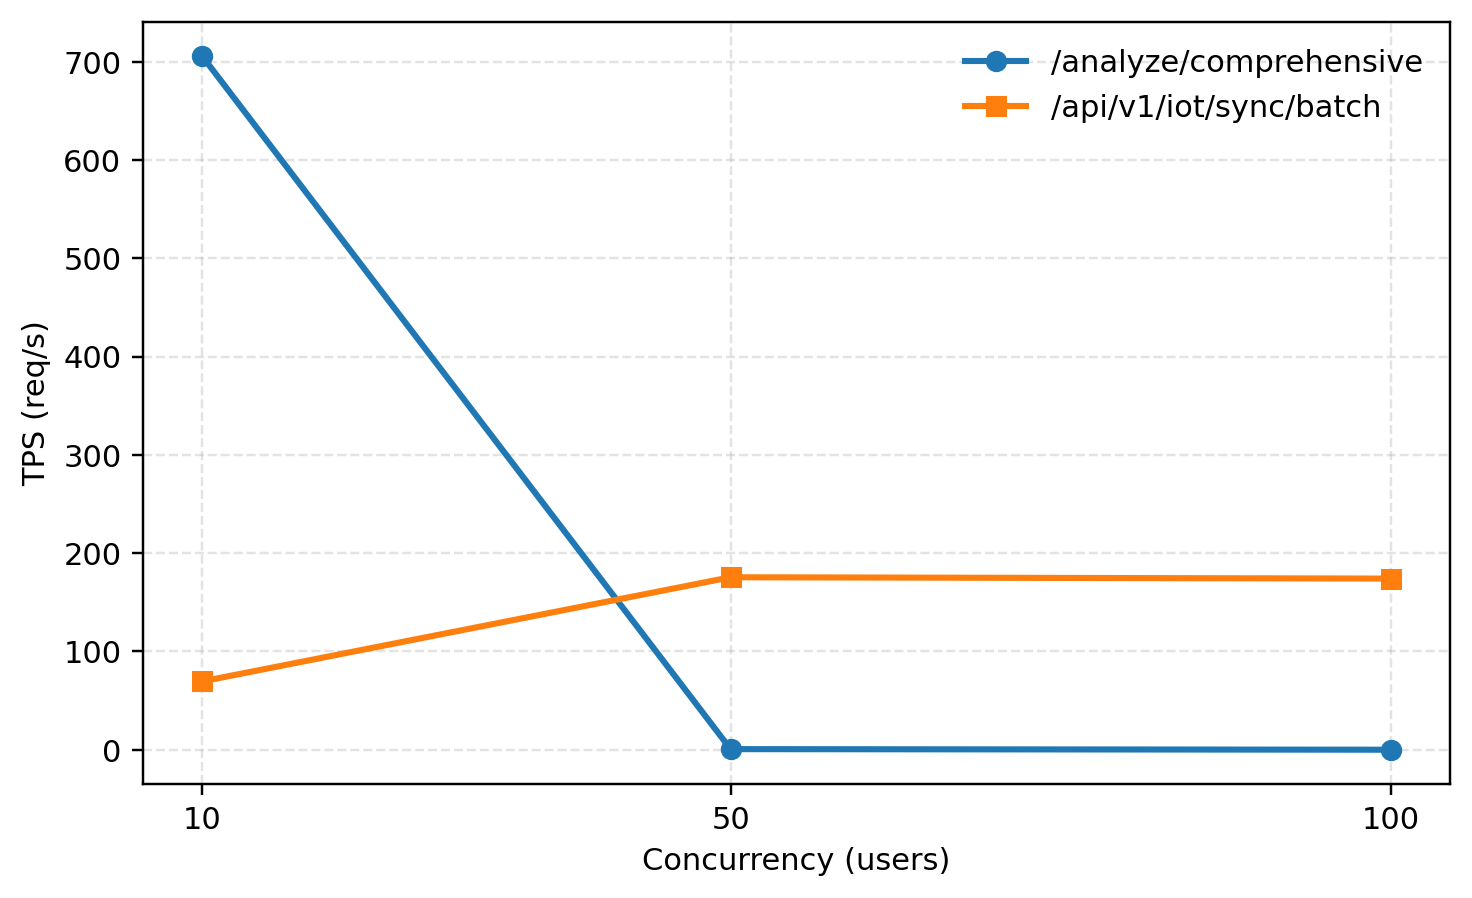
\includegraphics[width=0.88\textwidth]{fig_6_4_tps_concurrency}
\caption{核心接口 TPS-并发曲线。随着并发上升，\texttt{/api/v1/iot/sync/batch} 吞吐在中高并发段保持稳定平台；\texttt{/analyze/comprehensive} 在并发 50 后吞吐显著塌缩，表现为非线性退化。}
\label{fig:tps_curve_64}
\end{figure}

\begin{figure}[htbp]
\centering
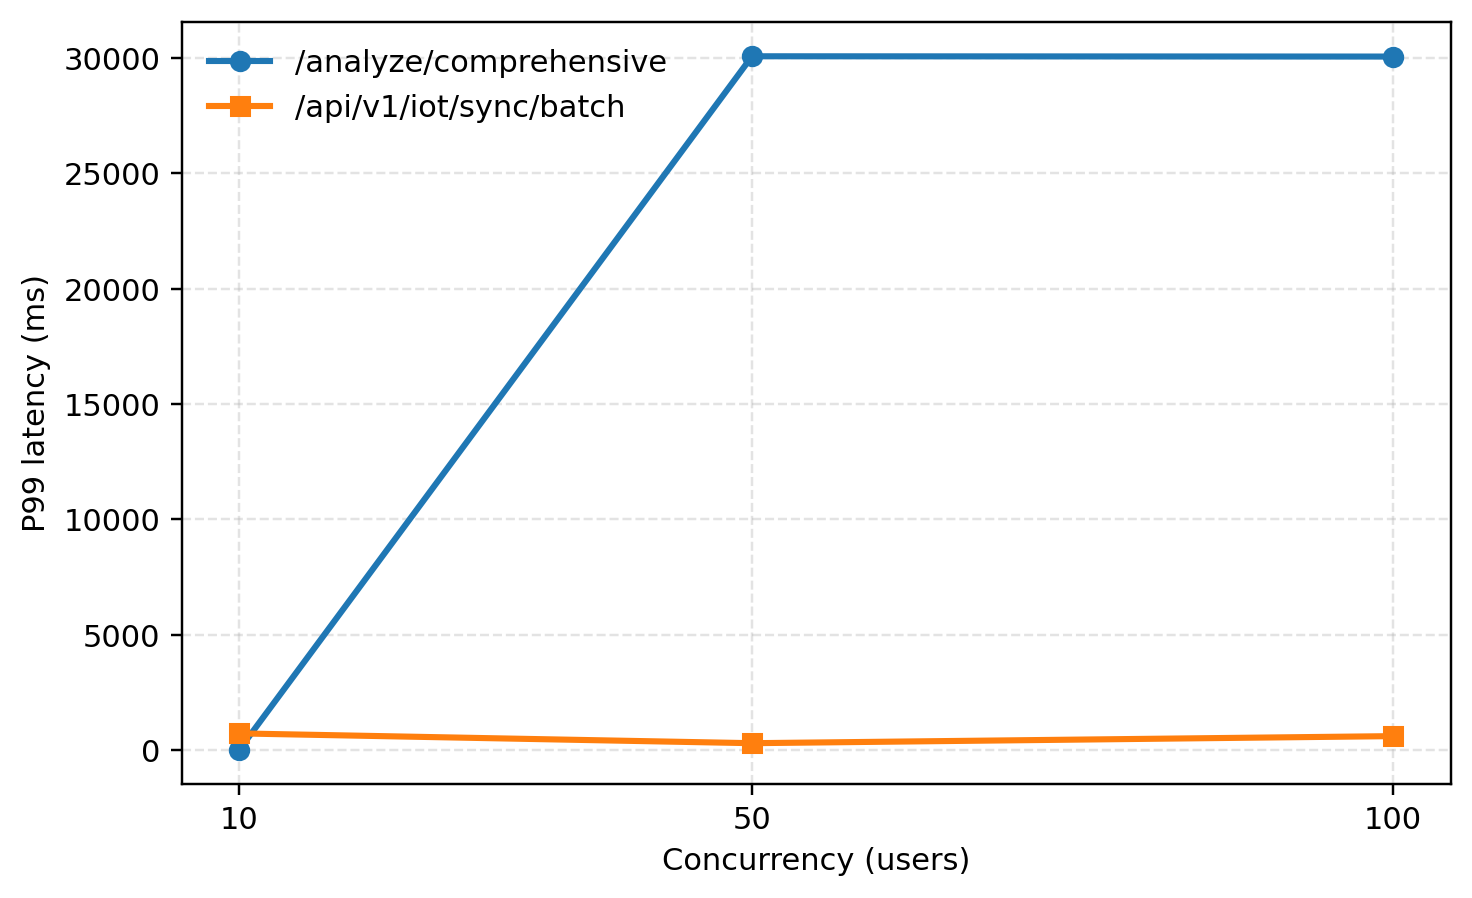
\includegraphics[width=0.88\textwidth]{fig_6_5_p99_concurrency}
\caption{核心接口 \(RT_{99}\)-并发曲线。\texttt{/analyze/comprehensive} 在并发 50/100 下出现 30s 级长尾，后端日志同步记录 \texttt{QueuePool timeout}，指向数据库连接池耗尽；\texttt{/api/v1/iot/sync/batch} 的 \(RT_{99}\) 维持在亚秒级。}
\label{fig:p99_curve_64}
\end{figure}

\subsection{缓存性能分析}
缓存实验聚焦对话链路 \texttt{/chat/send} 的性能收益与一致性代价。系统在生命周期启动阶段初始化 Redis 连接；当缓存不可用时自动降级为直连推理。性能收益采用加速比度量：
\begin{equation}
Speedup=\frac{RT_{\mathrm{no\_cache}}}{RT_{\mathrm{cache}}},
\end{equation}
并以命中率衡量缓存有效性：
\begin{equation}
HitRate=\frac{N_{\mathrm{hit}}}{N_{\mathrm{hit}}+N_{\mathrm{miss}}}.
\end{equation}
实验对照组分别为“缓存命中路径（\texttt{force\_refresh=False}）”与“强制回源路径（\texttt{force\_refresh=True}）”，用于量化秒级大模型调用向毫秒级缓存返回的时延压缩效果。

一致性验证采用状态机化链路追踪。触发事件 \(E_1\) 为用户调用 \texttt{/user/profile} 更新画像，触发事件 \(E_2\) 为用户调用 \texttt{/api/v1/ocr/upload} 导入新体检单。两类事件均调用 \texttt{CacheManager.invalidate\_user\_cache(user\_id)} 执行按用户粒度的失效清理。为保证失效模式可达，缓存键规范统一为 \texttt{chat\_response:\{user\_id\}:\{hash\}} 与 \texttt{diet\_plan:\{user\_id\}:\{hash\}}，与失效规则中的通配模式保持一致。

在时序层面，系统呈现“失效触发后首次回源重算、后续请求恢复命中”的可预期行为：首个请求承担一致性修复成本，随后命中率回升并重新进入低时延稳态。该机制实现了“以一次性局部延迟换取全域数据一致性”的工程折中，可有效避免旧病历或旧画像污染后续问答与干预建议。

\begin{table}[htbp]
\centering
\caption{缓存开启/禁用性能对比与加速比统计（\texttt{/chat/send}）}
\label{tab:cache_perf_64}
\begin{tabular}{lrrrr}
\toprule
实验模式 & 样本数 \(n\) & \(RT_{\mathrm{avg}}\) (ms) & \(RT_{99}\) (ms) & 指标 \\
\midrule
强制回源（\texttt{force\_refresh=True}） & 3 & 31699.18 & 33466.72 & 基线 \\
缓存命中（\texttt{force\_refresh=False}） & 8 & 2.04 & 2.46 & 命中率 100.00\% \\
\midrule
\multicolumn{5}{l}{加速比 \(Speedup = RT_{\mathrm{no\_cache}}/RT_{\mathrm{cache}} = 15511.11\times\)} \\
\bottomrule
\end{tabular}
\end{table}

\begin{figure}[htbp]
\centering
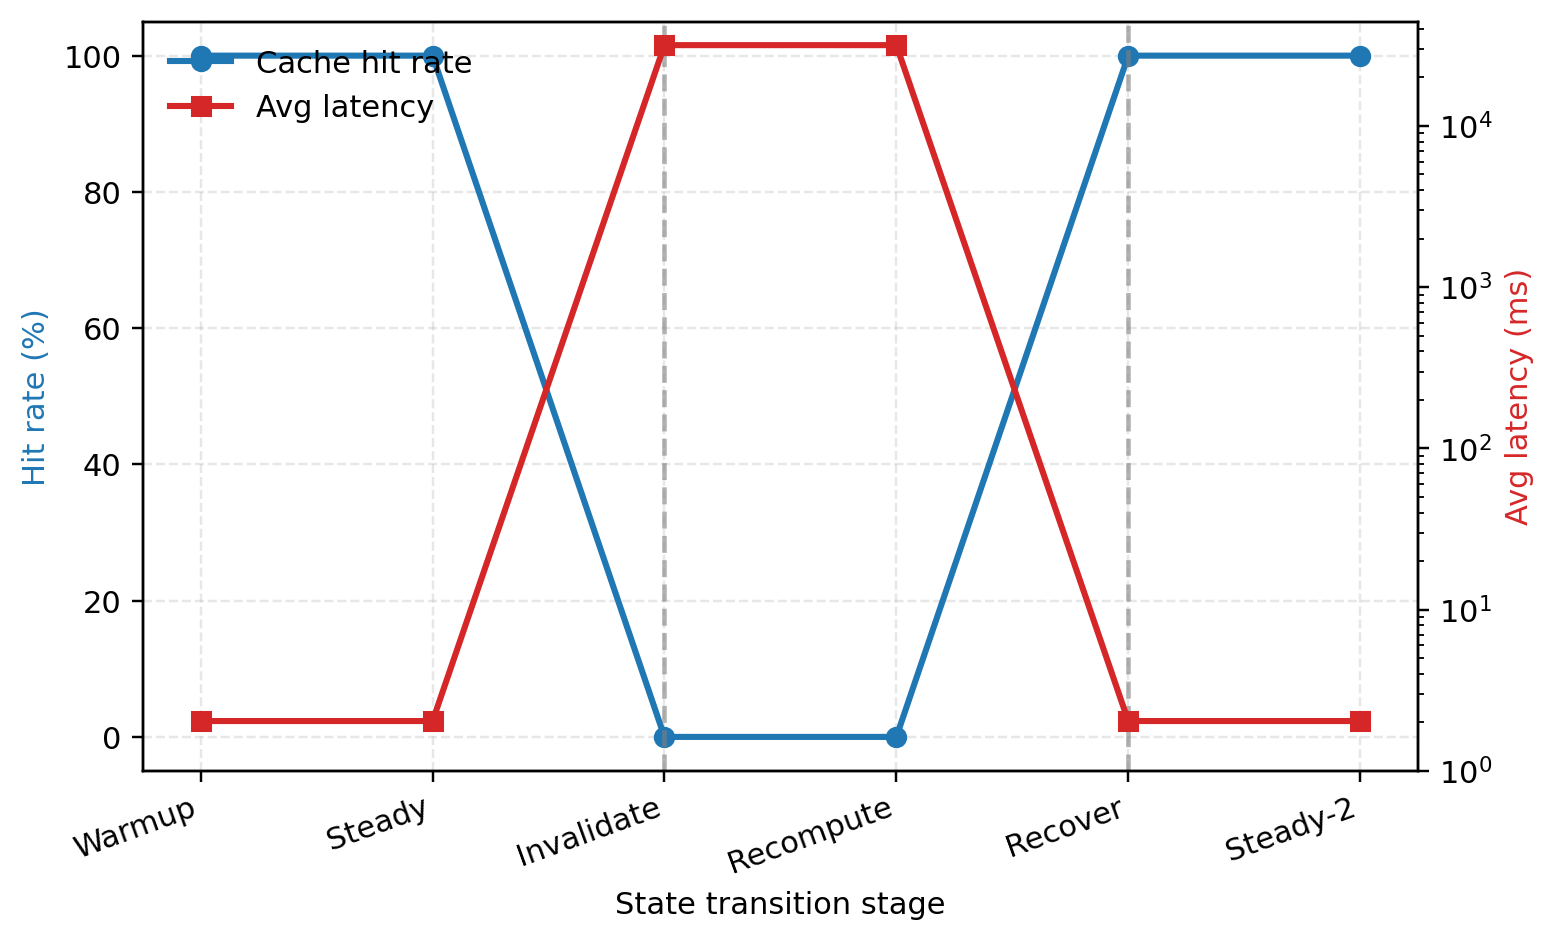
\includegraphics[width=0.88\textwidth]{fig_6_6_cache_timeline}
\caption{缓存命中率回落与恢复时序图。状态机顺序为“预热命中 \(\rightarrow\) 触发失效（画像更新/OCR 上传）\(\rightarrow\) 首次回源重算 \(\rightarrow\) 命中恢复”。实验日志显示缓存命中阶段响应时间从秒级降至毫秒级，验证了失效机制与缓存收益可以同时成立。}
\label{fig:cache_state_64}
\end{figure}

% !TeX root = ../main.tex
% ============================================
% 第七章 总结与展望
% ============================================

\chapter{总结与展望}

\section{工作总结}

本文完成的核心工作，是围绕主动健康管理场景构建一条从多模态输入组织、综合风险分析到情景推演与受控解释反馈的工程主链。针对多模态健康数据来源分散、风险分析链路不连贯以及智能问答缺乏受控约束等问题，论文完成了从理论基础、系统设计、算法建模到平台实现与实验验证的整体研究，并在统一框架下衔接了临床指标、遗传信息、文档解析结果、行为观测以及知识增强问答之间的关键关系。

从具体工作看，本文首先围绕主动健康管理平台的数据组织问题，完成了结构化临床指标、遗传信息、OCR 文档结果和行为观测信息的统一接入与管理，使后续分析能够建立在相对一致的输入基础上。在此基础上，本文设计并实现了以综合风险分析为中枢的主业务链，并在同一风险引擎基础上扩展了情景化推演能力，使平台不仅能够输出静态风险结果，还能够在当前实现边界内提供面向未来变化和干预方案的对比信息。进一步地，本文将受控 Agent 机制引入健康问答场景，通过意图分流、工具约束、证据门控、审计留痕和行为评测等机制，把问答过程限制在可追踪、可复核的运行框架内，使其承担分析结果的解释与反馈职责，而不是将其作为完全开放的生成式接口。

结合第 6 章的验证结果可以看到，当前平台已经具备较为完整的工程原型特征。训练脚本、服务逻辑和前端状态之间的主要输入边界能够保持一致，仓库级回归与浏览器场景测试也表明档案录入、OCR 状态回传、综合分析、历史会话管理和问答交互等关键链路在当前代码版本中可以稳定运行。与此同时，Agent 的受控 Harness 评测结果表明，其在固定场景下具备可回归、可审计的行为边界。总体而言，本文完成的是一套面向主动健康管理场景的工程化原型方案，其价值主要体现在把多模态风险分析、情景推演和受控问答组织成了一条可以落地验证的实现链路。

\section{不足与局限}

尽管本文已经完成多模态健康管理平台的原型构建与验证，但当前工作仍有比较明确的边界。首先，在数据与模型层面，真正高质量、长周期且完成临床表型、遗传风险和行为观测配对的真实世界数据仍然有限。当前风险建模、风险修正和情景推演更多体现为面向原型系统的工程验证，其泛化能力仍需在更大规模、更多样化的人群和场景中继续检验。尤其是第 6 章中已经说明，部分离线 benchmark 和更细粒度的消融排序并未在本轮环境下完整重跑，因此相关结论应当保持在实现基础和方法可行性的层面，而不能外推为充分的临床统计结论。

其次，在系统层面，本文实现的是一个可运行、可验证的轻量化平台原型，而不是面向大规模生产部署的终态架构。当前后端服务组织、异步任务处理、持久化方案和容器部署方式已经能够支撑论文验证与中低负载场景，但在更高并发、多用户和长时间在线运行条件下，仍可能面临资源占用、调度弹性和扩展能力方面的约束。此外，OCR 解析和问答生成均依赖外部 API 服务，其可用性、响应延迟、调用额度和隐私合规要求都会影响系统在真实环境中的稳定运行；真实运行环境下也可能先触发状态回传和待识别流程，而不是始终进入完整自动回填路径。后续若面向更严格的部署场景，还需要进一步完善本地化模型替代、请求脱敏、访问审计和服务降级策略。这些现象都说明，现有系统更适合作为平台设计思路和关键链路的验证载体，而不是直接面向复杂生产环境的最终方案。

最后，在 Agent 模块层面，本文所证明的主要是受控问答链路的工程可控性、审计可追踪性和行为一致性，而不是 Agent 在真实医疗场景中的全面临床有效性。意图分流、工具约束、证据门控和行为评测能够明显收紧系统回答边界，但这些机制并不能替代医生在复杂医学判断中的专业决策。因此，本文中的 Agent 更适合被理解为健康管理平台中的受控交互模块，而非具备独立诊疗能力的智能代理。

\section{未来展望}

后续工作首先需要继续积累更高质量的真实世界多模态健康数据，增强临床、遗传、文档与行为信息在同一主体下的长期配对能力。只有在数据覆盖度、时间跨度和标注质量进一步提升后，风险评估、风险修正和情景推演的结果才更有可能获得更稳健的统计支撑。与之对应，离线评测部分也需要进一步补足系统性的校准分析、跨人群比较和更加完整的消融实验，使模型层面的结论不再主要依赖工程侧的一致性验证。

在平台实现方面，后续工作可以在保持当前主业务链稳定的前提下，进一步增强 OCR 文档解析的鲁棒性、分析上下文的连续性以及多页面状态协同能力。对于问答模块，则更适合沿着“受控增强”而不是“能力泛化”的方向推进，在维持现有审计与约束机制的基础上，逐步提升工具利用效率、证据组织方式和人工接管协同能力。与此同时，平台若要进入更复杂的真实应用环境，还需要进一步补足隐私保护、权限治理、扩展部署和运行监测等工程能力。

总体来看，主动健康管理平台的持续发展不仅依赖模型能力增强，也依赖数据质量提升、系统工程完善和治理机制同步演进。本文完成的工作为这一方向提供了初步的工程化基础，但其更重要的意义仍然在于验证了一个可实现、可测试、可逐步扩展的技术路线。后续研究仍需要在真实应用环境中不断检验、修正并收紧其适用边界。


% ==================== 参考文献 ====================
\bibliography{references}

% ==================== 致谢（参照学长论文格式）====================
\chapter*{致\quad 谢}
\addcontentsline{toc}{chapter}{致\quad 谢}
在本论文完成之际，衷心感谢指导教师吴松老师在毕业设计期间给予的悉心指导与耐心帮助。

\end{document}
